\documentclass[10pt,journal,letterpaper]{IEEEtran}
\usepackage[T1]{fontenc}
\usepackage[utf8]{inputenc}
\usepackage{amsmath,amssymb,booktabs,graphicx,tabularx,microtype}
\usepackage{cite}
\usepackage[hidelinks]{hyperref}
\usepackage{placeins}
\interdisplaylinepenalty=2500
\emergencystretch=1.5em

% Retain natural table text size and shrink only when necessary.
\newsavebox{\ArticleTableBox}
\newcommand{\FitTable}[1]{%
  \sbox{\ArticleTableBox}{#1}%
  \ifdim\wd\ArticleTableBox>\linewidth
    \resizebox{\linewidth}{!}{\usebox{\ArticleTableBox}}%
  \else
    \usebox{\ArticleTableBox}%
  \fi
}

\renewcommand{\abstractname}{Resumen}
\renewcommand{\IEEEkeywordsname}{Palabras clave}
\renewcommand{\refname}{Referencias}
\renewcommand{\tablename}{Tabla}
\renewcommand{\appendixname}{Apéndice}
\hypersetup{pdftitle={Pronóstico de recursos de microservicios con telemetría incompleta: descomposición, modelos compactos y transferencia calibrada},pdfauthor={Carlos Augusto Mullisaca Condori; Jhon Alex Gutiérrez Morales}}
\title{Pronóstico de recursos de microservicios con telemetría incompleta: descomposición, modelos compactos y transferencia calibrada}
\author{Carlos~Augusto~Mullisaca~Condori y Jhon~Alex~Gutiérrez~Morales%
  \thanks{Escuela Profesional de Ingeniería de Sistemas, Facultad de Ingeniería y Arquitectura, Universidad Peruana Unión, Juliaca, Perú. Correos: \mbox{\nolinkurl{carlos.mullisaca@upeu.edu.pe}} y \mbox{\nolinkurl{alex.gutierrez@upeu.edu.pe}}. Autor correspondiente pendiente de designación.}}

\begin{document}
\maketitle
\begin{abstract}
La telemetría incompleta dificulta el pronóstico de recursos de microservicios y puede modificar la precisión que se obtiene al aumentar la complejidad de los modelos. Se examina cómo la descomposición temporal, los descriptores de disponibilidad y el tamaño del modelo afectan al pronóstico de CPU y memoria en cinco fases. El experimento histórico ChronoGraph utiliza 28 servicios, 8005 instantes, división cronológica 70/10/20, historias de doce pasos, tres semillas y veinte máscaras emparejadas. Las variantes E0--E5 y C0--C3/V2 motivan la transferencia calibrada a 32 servicios adicionales. La ampliación compara quince familias con diez semillas neuronales y veinte máscaras. Los experimentos secundarios varían la ausencia, los horizontes directos y las historias. Los modelos congelados se transfieren a un día de Alibaba 2022 tras seis horas de calibración. Históricamente, E5 reduce el MASE emparejado de memoria en 1.280\% frente a DLinear y aumenta el de CPU en 0.984\%. V2 no conserva toda la mejora en memoria. En los servicios adicionales, A3 usa 15 parámetros y mejora el MASE de memoria en 0.02523 frente a E5, de 74 parámetros. Las diez medias por semilla favorecen A3 (prueba exacta de signos con $p=0.0078125$ ajustada por Holm), con mejora en solo 10 de 32 servicios. A3 no mejora de forma general frente a DLinear. PatchTST pequeño y NLinear obtienen las menores medias principales, y persistencia lidera el caso externo. A3 registra medianas CPU/CUDA de 0.050/0.141 ms con entradas residentes para un origen y 32 servicios. Los compromisos observados dependen de las pérdidas sintéticas, los períodos compartidos y la corta evaluación externa.

\end{abstract}
\begin{IEEEkeywords}
Microservicios, pronóstico, telemetría incompleta, DLinear, transferencia calibrada, reproducibilidad.
\end{IEEEkeywords}

\section{Introducción}
Los pronósticos de CPU y memoria pueden aportar información a la planificación de capacidad y al autoescalado de microservicios. Una arquitectura de microservicios distribuye funcionalidades entre componentes que se comunican mediante llamadas; sus mediciones temporales y relaciones permiten estudiar tanto la historia local como información del entorno. Sin embargo, pronosticar el uso registrado no equivale a estimar demanda sin restricciones ni demuestra que un controlador asigne mejor los recursos. Los trabajos sobre aprendizaje de cargas, autoescalado y pronóstico de recursos ofrecen el contexto aplicado \cite{powerprediction,autoscaling2025,temposcale,aero}. Este estudio evalúa errores puntuales y ejecución de modelos, sin medir energía, facturación o cumplimiento de acuerdos de servicio.

La telemetría puede faltar cuando fallan la recolección, el transporte o los servicios. El predictor debe distinguir el último valor conocido de una medición nueva. El problema inicial fue modificar un modelo ligero para representar esa procedencia y cambiar su descomposición temporal. Un escalar imputado permite ejecutar el modelo, pero no identifica el proceso de observación. Añadir características de ausencia puede ayudar a interpretar la historia y también incrementar capacidad, redundancia o ajuste al generador sintético. Su utilidad requiere evidencia de error y coste, no solamente una justificación semántica.

DLinear combina proyecciones afines de una componente móvil y su residual \cite{dlinear}. Cuando el suavizamiento es una transformación lineal fija, la suma sigue siendo una función afín de la ventana. Reducir su parametrización no crea necesariamente una nueva clase funcional. El suavizamiento dependiente de disponibilidad y las características explícitas de ausencia constituyen intervenciones distintas. Ni una equivalencia algebraica ni un menor número de parámetros garantizan mejorar la predicción. Esta distinción motivó pasar del estudio de descomposición a modelos compactos y, después, a referencias más amplias.

La investigación integra cinco fases complementarias. La fase I evalúa E0--E5 y comparadores originales sobre 28 servicios de ChronoGraph. La fase II estudia C0--C3 y la regla V2 seleccionada mediante validación, sobre la misma prueba conocida. La fase III vuelve a ajustar modelos fuente con el protocolo ampliado y los transfiere a 32 servicios adicionales. La fase IV añade mecanismos de pérdida, horizontes directos, ventanas y un caso externo de Alibaba 2022. La fase V mide el coste de las implementaciones. La secuencia desarrolla una pregunta común; las fases no son réplicas independientes ni sus errores se suman.

El resultado histórico favorable de E5 en memoria motivó desarrollos posteriores. Los cuatro contrastes principales se congelaron localmente antes de evaluar los servicios destino, aunque el período fuente ya era conocido. Los servicios adicionales comparten infraestructura y período con la fuente: constituyen transferencia espacial calibrada, no una replicación temporal cegada. Los protocolos y pesos congelados mejoran la transparencia del procedimiento, pero no convierten toda la investigación en un ensayo prospectivo independiente ni equivalen a un prerregistro público.

La brecha abordada es una evaluación conjunta y trazable de descomposición, procedencia de mediciones, capacidad, coste y transferencia. La contribución es empírica: una parametrización afín compacta con dos descriptores separados, comparación emparejada de quince familias bajo diez condiciones, extensiones de horizonte y ventana, transferencia externa calibrada, reconstrucción de métricas y mediciones de inferencia CPU/CUDA. Se conservan resultados negativos y cambios de clasificación. La contribución no consiste en afirmar que una arquitectura resuelve universalmente la gestión de recursos.

\subsection{Preguntas de investigación y alcance}
La pregunta central es cómo afectan la descomposición temporal, la representación de telemetría incompleta y la complejidad a precisión, robustez, eficiencia y transferencia del pronóstico. Se concreta en seis preguntas: PI 1, cómo cambia el error al perder observaciones; PI 2, qué compromiso produce la descomposición fija, el suavizamiento dependiente de disponibilidad y la parametrización compacta; PI 3, cuándo ayudan la fracción ausente y la edad; PI 4, si un modelo afín compacto conserva precisión con menos parámetros; PI 5, cómo cambian las conclusiones entre servicios, horizontes y dominios; y PI 6, cuánta variación aparece entre inicializaciones, máscaras y períodos.

La hipótesis principal compara A3 con DLinear y E5 para CPU y memoria mediante cuatro contrastes bilaterales. La finalización no exige obtener una mejora. La monotonía frente a pérdidas, las ablaciones, mecanismos añadidos, ventanas, horizontes y transferencia externa son análisis secundarios descriptivos. La evidencia histórica es exploratoria y genera hipótesis. Un efecto puede conservar dirección entre inicializaciones y concentrarse en pocos servicios, por lo que consistencia entre semillas, portabilidad y tamaño del modelo se interpretan separadamente. La Fig.~\ref{fig:flow} muestra el flujo de selección y evaluación.
\begin{figure*}[!t]\centering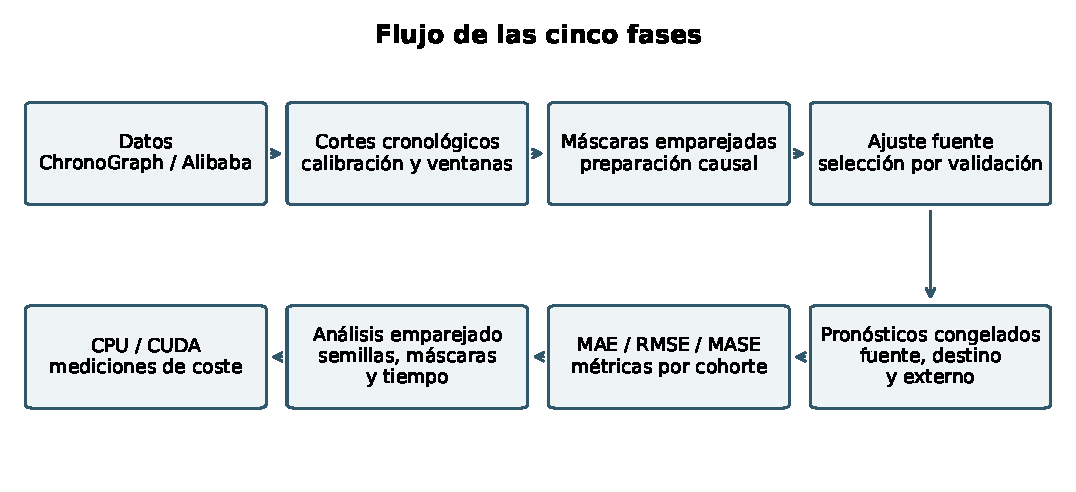
\includegraphics[width=0.93\textwidth]{figuras/es_01_methodology.pdf}
\caption{Flujo experimental. La selección y los pesos usan entrenamiento y validación de los 28 servicios fuente. Los 32 servicios destino aportan estadísticas de calibración del prefijo, sin ajuste de pesos. Alibaba utiliza un prefijo separado de seis horas.}\label{fig:flow}
\end{figure*}

\section{Trabajos relacionados y fundamentos teóricos}
Las referencias lineales son necesarias al comparar modelos temporales profundos. DLinear y NLinear cuestionan que la complejidad arquitectónica explique por sí sola la precisión \cite{dlinear}. PatchTST usa parches independientes por canal \cite{patchtst}; TimesNet representa variación temporal en dos dimensiones \cite{timesnet}; iTransformer utiliza variables como dimensión de los elementos de atención \cite{itransformer}; TiDE emplea codificación densa \cite{tide}; y TimeMixer combina escalas temporales \cite{timemixer}. Estos trabajos tienen presupuestos y protocolos distintos. Aquí se ejecuta una configuración pequeña de PatchTST basada en código oficial; las otras cuatro arquitecturas son antecedentes bibliográficos, sin resultados experimentales propios en la cola ampliada.

Un dataset multivariante no obliga a que cada predictor utilice todas las variables conjuntamente. CPU y memoria son objetivos separados. La mayoría de modelos lineales comparte coeficientes entre servicios, pero consume la historia de un recurso de un servicio, normalizada con estadísticas propias. La GRU de grafo agrega vecinos. Por ello, una proyección univariante compartida no debe describirse como un modelo conjunto aprendido de toda la infraestructura. NLinear resta el último valor preparado, proyecta la historia centrada y vuelve a añadir ese valor; bajo ausencia, ese nivel reciente puede ser una imputación arrastrada, sin recuperación del dato oculto.

Una descomposición separa nivel suavizado y residual \cite{hyndmanfpp3}. El residual no demuestra estacionalidad, y una autocorrelación diaria tampoco basta para identificarla. MA25 repite extremos cuando opera sobre doce posiciones, de modo que el relleno forma parte del método. La componente exponencial actualiza un estado y la variante consciente de disponibilidad omite actualizaciones imputadas. Persistencia, media móvil y suavizamiento exponencial se evalúan también como predictores directos. Compartir una recurrencia no hace equivalentes un suavizador estadístico y una descomposición interna seguida de pesos entrenados.

Las GRU resumen secuencias mediante estados y compuertas \cite{gru}. GRU-D incorpora indicadores y decaimiento \cite{grud}; aquí se adapta a pesos compartidos entre servicios, sin reproducir su experimento clínico. BiTGraph y GinAR consideran estructuras temporales, relaciones y datos faltantes \cite{bitgraph,ginar}. Sus resultados históricos se preservan, incluso errores extremos, pero no se ajustan nuevamente en todos los escenarios. Las GRU local y de grafo amplían la comparación mediante información propia y agregados de llamadas. Una adyacencia estática conocida no demuestra influencia causal ni disponibilidad de cada arista en cada instante.

La imputación causal completa la entrada numérica; los indicadores registran si fue observada, arrastrada o reemplazada por mediana. La edad puede resumir una observación anterior al inicio de la ventana explícita. Rubin distingue los mecanismos de ausencia por la información de la que depende la disponibilidad \cite{rubinmissing}. El mecanismo sintético MAR dependiente del retardo vincula disponibilidad con CPU observada previamente, sin utilizar CPU contemporánea oculta. Su ejecución no prueba que las averías reales sigan MAR. La redundancia entre indicadores y edad también limita la interpretación aislada de coeficientes.

Los trabajos aplicados distinguen el objetivo predictivo y la acción posterior. TempoScale estudia predicción relacionada con autoescalado \cite{temposcale}, AERO combina predicción y orquestación \cite{aero}, y STAMP incorpora estado y dependencias espaciotemporales \cite{stamp}. Las revisiones de técnicas para microservicios y autoescalado sitúan estas contribuciones \cite{aimapping,autoscaling2025}. La RSL reciente de los autores aportó referencias candidatas; sus publicaciones primarias se verificaron antes de inclusión. El número de artículos de esa RSL no representa experimentos ejecutados aquí. Los trabajos sobre variables ausentes, muestreo dinámico, gestión adaptativa y anomalías aportan contexto adicional con su estado de publicación registrado \cite{ibn,radar2026,taxonomy2026,ibm2026}. Sus puntuaciones de anomalías no se comparan con MASE.

STEAM construye un grafo a partir de similitudes de carga y utiliza información del estado del sistema para obtener vistas alternativas del grafo \cite{steamgraph}. Este diseño permite contextualizar la adyacencia estática de llamadas que usamos aquí. DeepScaling evalúa una política de escalado orientada a estabilizar la utilización de CPU \cite{deepscaling}. Su evaluación incluye decisiones de control, mientras que este estudio mide el error de pronóstico sobre el uso registrado.

La incertidumbre de una diferencia media entre algoritmos es distinta de la incertidumbre de una futura observación. Los intervalos aquí remuestrean comparaciones bajo dependencia temporal \cite{blockbootstrap}; no son intervalos predictivos ni prueban cobertura. La predicción conforme requiere supuestos y calibraciones adicionales \cite{conformal}. MASE normaliza por variación del prefijo de entrenamiento \cite{mase}, pero no elimina diferencias semánticas entre CPU, memoria y utilización normalizada externa. La Tabla~\ref{tab:related} delimita el alcance implementado.
\begin{table*}[!t]
\caption{Estado del arte y alcance implementado. No se combinan resultados publicados en tareas distintas con las mediciones presentes.}\label{tab:related}
\centering\footnotesize
\begin{tabularx}{\linewidth}{p{.22\linewidth}XX}
\toprule Trabajo/familia & Mecanismo pertinente & Ejecución y límite \\\midrule
DLinear/NLinear \cite{dlinear} & Pronóstico afín y tratamiento del nivel & Ejecutados; historias cortas y selección fuente \\
GRU/GRU-D \cite{gru,grud} & Compuertas, disponibilidad y decaimiento & Adaptaciones ejecutadas; tarea clínica no reproducida \\
BiTGraph/GinAR \cite{bitgraph,ginar} & Grafos y variables incompletas & Solo históricos; presupuesto y tarea locales \\
PatchTST \cite{patchtst} & Parches temporales independientes por canal & Configuración pequeña ejecutada \\
TimesNet, iTransformer, TiDE, TimeMixer \cite{timesnet,itransformer,tide,timemixer} & Representaciones temporales alternativas & Solo revisados, sin clasificación experimental local \\
Predicción en nube \cite{powerprediction,temposcale,aero,stamp} & Integración con gestión de recursos & Contexto; no se midieron resultados de control \\
\bottomrule\end{tabularx}
\end{table*}

\section{Metodología}
\subsection{Diseño, procedencia y separación de evidencia}
El estudio es computacional, cuantitativo y experimental, con evaluación cronológica de origen móvil. La descripción del error corresponde a servicio, recurso, condición, inicialización y realización de máscara. Las ventanas se solapan y los servicios comparten infraestructura. Una fila de resultados no equivale a una réplica independiente. La fase histórica es exploratoria; el escenario principal ampliado contiene cuatro contrastes preespecificados localmente. Los restantes análisis se presentan descriptivamente. La Tabla~\ref{tab:master} relaciona sus unidades y presupuestos.

El histórico contiene 8005 filas temporales compartidas, dos recursos y 28 servicios, con historia 12 y horizonte de un paso, equivalente a treinta minutos. Utiliza tres semillas, veinte máscaras y siete condiciones: datos completos y pérdidas dispersas o por bloques de 10, 20 y 40\%. Se conservan E0--E5, C0--C3, V2 y comparadores originales. V2 selecciona una familia compacta entrenada mediante validación; no es un modelo ajustado de forma independiente. La auditoría comprueba manifiestos y archivos preservados. No se combinan sus errores con los nuevos como si fueran repeticiones independientes.

ChronoGraph publica series nominalmente semihorarias y relaciones de llamadas \cite{chronograph}. El grafo publicado contiene 708 servicios y 1529 aristas. Los subconjuntos analizados no implican ajustar sobre los 708 servicios. Los cortes son $[0, 5603)$, $[5603, 6404)$ y $[6404, 8005)$:70/10/20 por filas, con redondeo. Existe un salto de 108000 segundos después de la fila 5907, dentro de validación. Ventanas y pares consecutivos del denominador MASE no atraviesan ese hueco. Para L12/H1 existen 5591 orígenes de entrenamiento, 777 de validación y 1589 de prueba históricos. La cohorte fuente es de conveniencia; el subgrafo histórico conserva 28 aristas internas y excluye 137 de frontera según la auditoría.

La cohorte destino de 32 servicios se elige mediante topología estática y recorrido reproducible ordenado por SHA, excluyendo los 28 originales y cuatro pilotos conocidos. No utiliza errores predictivos. Su conexión topológica y selección de conveniencia limitan la representatividad poblacional. Los pesos e hiperparámetros usan solo entrenamiento/validación fuente. Para cada servicio destino, sus primeras 5603 filas aportan media, desviación, mediana y denominador MASE. La validación destino no selecciona modelos. Se trata de transferencia espacial calibrada, no de pronóstico sin datos previos del destino. La CPU conserva la escala publicada y la memoria se mide en bytes; no se convierte CPU arbitrariamente a porcentaje o núcleos. El modelo de grafo recibe nuevas matrices de adyacencia, sin aprender pesos destino. No se estableció completamente la fecha de disponibilidad de cada arista.

El caso externo utiliza los primeros 48 objetos oficiales \texttt{MSMetricsUpdate} de Alibaba 2022, correspondientes a un día \cite{alibaba2022}. Una cola limitada verifica Content-MD5 del propietario y registra SHA256. Se descargaron 17890753336 bytes con 675424445 filas CSV de pods. Entre los servicios con cobertura de todos los instantes del primer objeto se eligen 32 por orden SHA y se ordenan lexicográficamente. La selección atiende a disponibilidad, no a precisión. Para cada instante se promedian pods por servicio con ambos recursos finitos; después se promedian esos instantes con el mismo peso dentro del intervalo semihorario. Un intervalo con menos de treinta observaciones de minuto válidas se considera ausente y solo queda disponible al cierre.

Alibaba publica utilización normalizada min--max, no núcleos ni bytes. El alcance temporal de esa normalización no está documentado aquí. Los 48 intervalos procesados se dividen en 12 de calibración, seis horas, y 36 objetivos, dieciocho horas. Cuatro valores escalares naturalmente ausentes se encuentran solo en calibración, dos pares servicio/intervalo en ambos recursos. Ningún objetivo externo se imputa. Los pesos fuente L12/H1 permanecen congelados, sin ajuste ni selección externa. Se excluye GRU de grafo porque no se adquirió la red de llamadas externa. Este diseño no aplica 70/10/20 a Alibaba y constituye un caso exploratorio corto.

\subsection{Preparación causal, normalización y máscaras}
Sea $ y_{t,s,r}$ la medición de recurso $ r $, servicio $ s $ e instante $ t $. Cada recurso se pronostica por separado. Una entrada de $ L $ pasos termina en $ t-h $ y produce directamente el objetivo $ y_{t,s,r}$. Los límites de partición y huecos reinician la preparación. Se calcula $ x=(y-\mu)/\max(\sigma, 10^{-8})$ con estadísticas del prefijo correspondiente; la inversión devuelve $\widehat y=\sigma_*\widehat x+\mu $. Las estadísticas de calibración preceden las máscaras sintéticas. Por ello no se evalúa aprender esas estadísticas a partir de un prefijo artificialmente degradado.

Una medición disponible se conserva; cuando falta, se arrastra la última observación del segmento y, antes de la primera, se usa la mediana de entrenamiento. El indicador observado es $ m $, el de ausencia después de observar es $ c $ y el de respaldo por mediana es $ f $, con $ m+c+f=1$. La edad satisface $\delta_i=(1-m_i)(\delta_{i-1}+1)$ y comienza en cero antes del segmento. Si no hubo observación dentro de este, mide la racha desde el corte, no un tiempo real desconocido anterior. Los canales contienen valor normalizado preparado, $ m $, edad $\log(1+\delta)/\log(1+L)$, $ c $ y $ f $. El arrastre y la edad pueden resumir una observación anterior a la ventana explícita; $ L $ no limita estrictamente toda la información histórica.

Las siete condiciones originales conservan cantidades redondeadas exactas de ausencias por servicio y segmento. El patrón disperso selecciona entradas; el de bloques usa candidatos de hasta seis pasos. Se comparten máscaras entre métodos y recursos, y los objetivos originales permanecen disponibles para evaluación. El caso completo se cuenta una vez. Las tasas históricas son anidadas. Tres condiciones adicionales con etiqueta nominal 20\% incluyen pérdidas correlacionadas en grupos consecutivos de ocho servicios lexicográficos, bloques prolongados candidatos de hasta 24 pasos y MAR dependiente del retardo. La construcción de bloques deja separadores y puede truncar el último bloque para alcanzar el conteo exacto. Estas estructuras se imponen; no son interrupciones registradas.

La probabilidad MAR implementada es
\begin{equation}
 p_t=0.2\{1+0.5\tanh(|z^{\mathrm{CPU,ultima}}_t|)\},
\end{equation}
donde $ z^{\mathrm{CPU,ultima}}_t $ utiliza exclusivamente CPU observada previamente. Por tanto,$0.2\leq p_t<0.3$:20\% es una etiqueta nominal. La máscara compartida se intersecta con disponibilidad natural. El principal utiliza veinte semillas de máscara emparejadas entre modelos y entrenamientos. Esa secuencia se había usado históricamente; cambiar de servicios no la convierte en inédita. Las Figs.~\ref{fig:masks} y~\ref{fig:temporal} muestran los mecanismos y la preparación temporal.

\begin{figure*}[t]\centering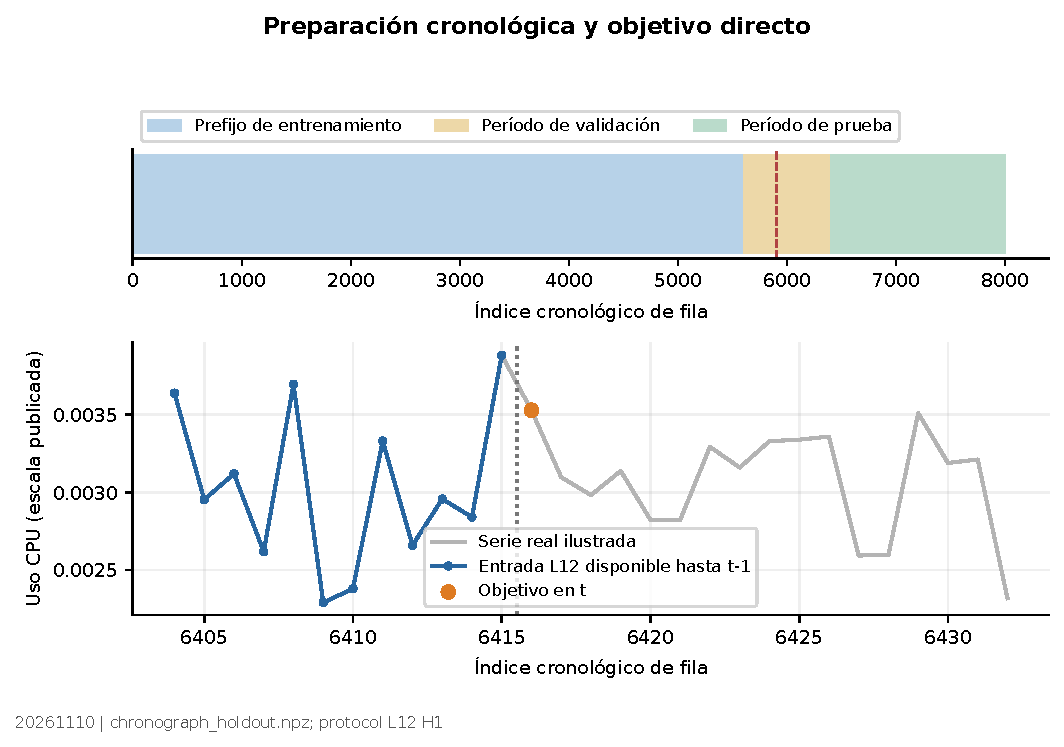
\includegraphics[width=0.72\textwidth]{figuras/es_04_temporal_preparation.pdf}
\caption{Cortes por filas y hueco de validación después de 5907. El ejemplo inferior usa valores reales L12/H1; el contexto posterior gris queda excluido de la entrada.}\label{fig:temporal}\end{figure*}

\begin{figure*}[t]\centering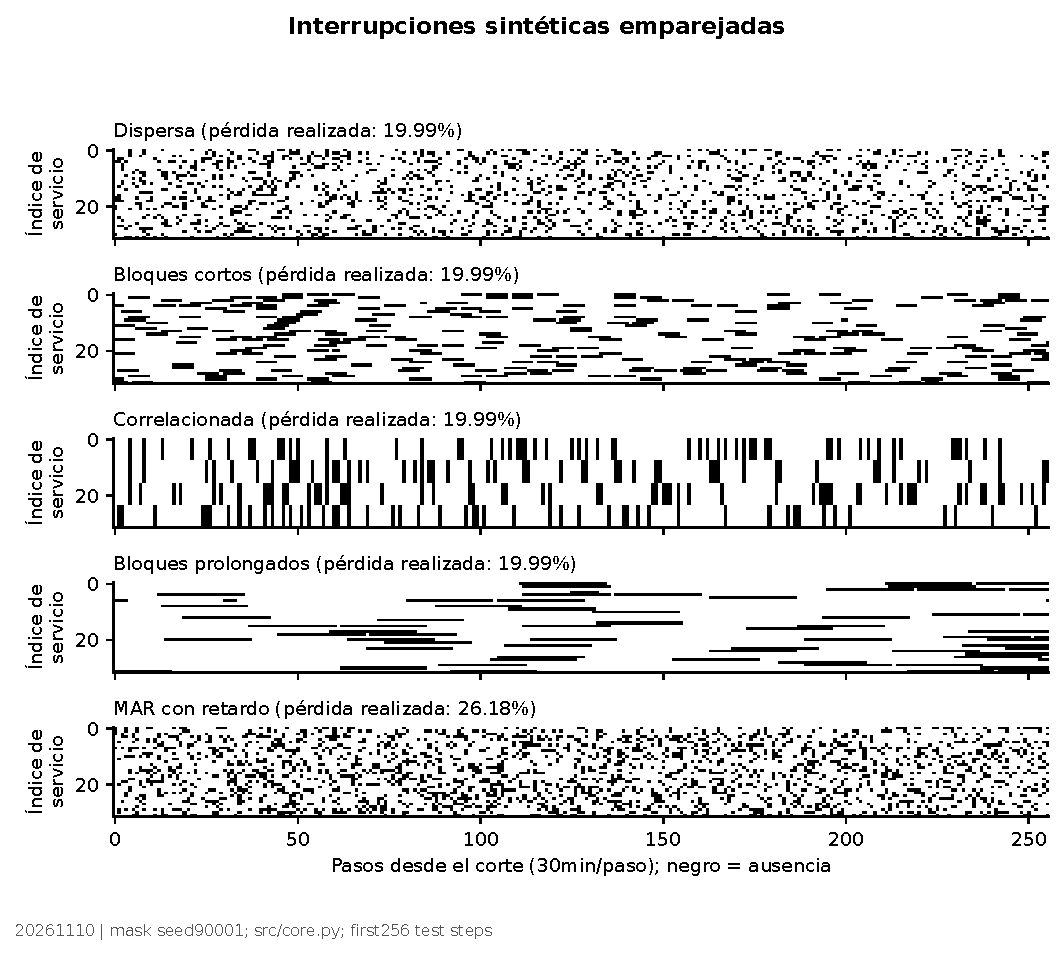
\includegraphics[width=0.68\textwidth]{figuras/es_05_missingness.pdf}
\caption{Máscaras efectivas, semilla 90001 y primeros 256 pasos de prueba. Negro indica ausencia. Correlación y duración son mecanismos impuestos; MAR no afirma 20\% exacto.}\label{fig:masks}\end{figure*}

\subsection{Descomposición histórica y familias compactas}
Para una ventana $ v\in\mathbb R^L $ y una matriz lineal fija de suavizamiento $ S $, DLinear calcula
\begin{align}
\widehat x&=w_t^\top Sv+w_r^\top(I-S)v+b_t+b_r\\
&=[S^\top w_t+(I-S)^\top w_r]^\top v+(b_t+b_r).
\end{align}
E0 utiliza MA25 con extremos replicados incluso cuando L12. El promedio centrado usa posiciones posteriores dentro de la historia, pero ninguna medición futura respecto del origen final. El residual no es una componente estacional demostrada. La transformación fija y la cabeza colapsada representan la misma clase afín; Adam y la regularización pueden seguir trayectorias diferentes. La Fig.~\ref{fig:dlinear} muestra esa distinción.

E1 selecciona ancho 3, 7, 13 o 25. E2 usa una componente exponencial inicializada por $\ell_1=v_1$:
\begin{equation}
\ell_i=\ell_{i-1}+\alpha m_i(v_i-\ell_{i-1}),\qquad r_i=v_i-\ell_i.
\end{equation}
Una imputación no actualiza el nivel como medición nueva. La búsqueda histórica consideró factores fijos 0.1, 0.3, 0.7 y un escalar aprendido mediante sigmoide; las selecciones finales emplearon factores fijos. E3 agrega una proyección sin sesgo de los 36 indicadores de procedencia; E4 proyecta doce edades; E5 combina EMA y ambas cabezas. Sus tamaños con factor fijo son 62, 38 y 74 parámetros frente a 26 de E0/E1/E2. Las cabezas añadidas comienzan en cero. Los indicadores colineales y la edad no son factores informativos ortogonales ni permiten interpretar coeficientes causalmente.

C0--C3 conservan dos cabezas de valor y añaden hasta dos coeficientes escalares:
\begin{equation}
\widehat x_C=\widehat x_{base}+\gamma_p L^{-1}\sum_i(1-m_i)+\gamma_a a_L.
\end{equation}
C0 no añade ninguno, C1 usa fracción ausente, C2 edad final y C3 ambos. Sus tamaños son 26, 27, 27 y 28. Seleccionan MA25, EMA0.3 o EMA0.7. V2 elige una familia por recurso mediante el promedio del mejor MASE de validación de tres ajustes, con desempate por tamaño e identificador. Reutiliza pesos y predicciones; no consulta objetivos futuros ni selecciona por servicio. C3 y V2 no son nombres alternativos de A3.

A0 colapsa las cabezas fijas de DLinear a una proyección afín. A1 agrega $ u=L^{-1}\sum_i(1-m_i)$, A2 la edad logarítmica final $ a=\log(1+\delta_{final})/\log(1+L)$, y A3 ambas:
\begin{equation}
\widehat x_{A3}=w^\top v+b+\gamma u+\eta a.
\end{equation}
Los tamaños son $ L+1,L+2,L+2,L+3$, frente a $2L+2$ de DLinear. A0--A3 inicializan el valor desde las mismas cabezas DLinear sembradas y comienzan los coeficientes adicionales en cero. La equivalencia float 32 inicial se verifica con tolerancias relativa $10^{-5}$ y absoluta $10^{-6}$, no igualdad bit a bit. La edad A no se recorta. Cada familia se selecciona independientemente, por lo que su comparación no mantiene hiperparámetros idénticos. E5 ampliado conserva $\alpha=0.7$ y edad lineal acotada; su descomposición depende de la máscara y queda fuera del colapso fijo. La Fig.~\ref{fig:a3} ilustra A3 y la Fig.~\ref{fig:evolution} sitúa las familias.

\begin{figure*}[!t]\centering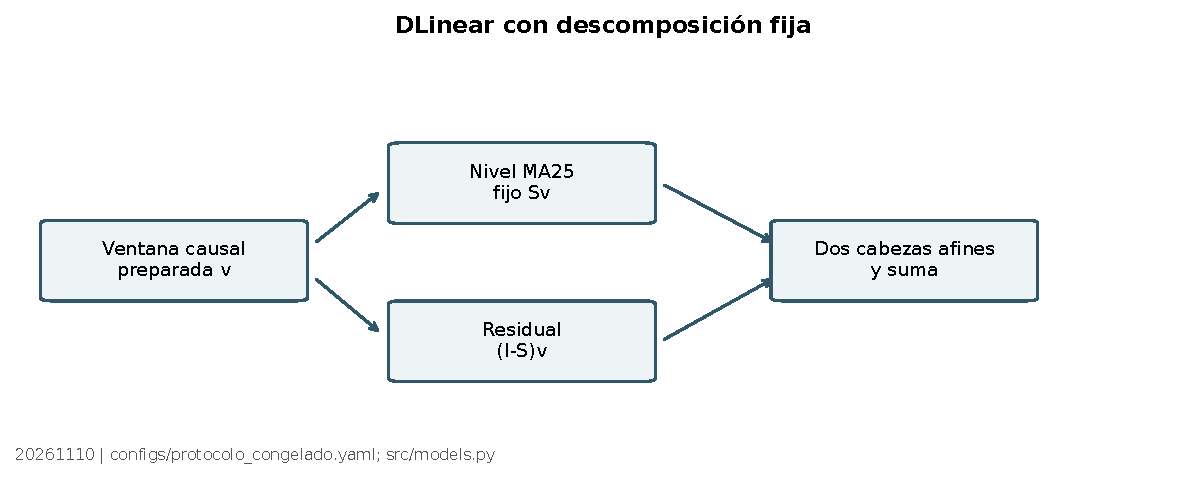
\includegraphics[width=0.79\textwidth]{figuras/es_02_dlinear.pdf}
\caption{Descomposición DLinear fija. Ambas componentes usan la historia disponible. El colapso afín no garantiza trayectoria de optimización idéntica.}\label{fig:dlinear}\end{figure*}

\begin{figure*}[!t]\centering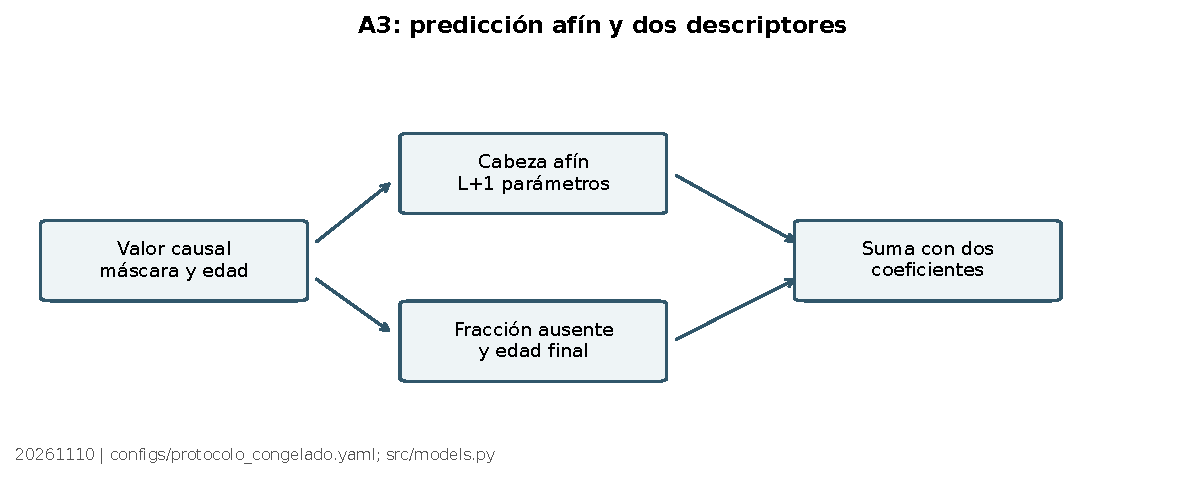
\includegraphics[width=0.79\textwidth]{figuras/es_03_a3.pdf}
\caption{A3 suma fracción ausente y edad logarítmica final a una cabeza afín. L12 requiere 15 parámetros por recurso; los coeficientes adicionales comienzan en cero.}\label{fig:a3}\end{figure*}

\subsection{Comparadores implementados}
Las referencias estadísticas son persistencia, media móvil y suavizamiento exponencial. Los candidatos de media son 1, 3, 6 y 12 pasos incluso con historias mayores. El suavizador actualiza solo con mediciones disponibles y considera $\alpha\in\{0.1, 0.3, 0.7, 0.9\}$. Ridge incluye intercepto no penalizado y $\lambda\in\{0, 10^{-4}, 10^{-2}, 1\}$, con ajuste analítico sobre las diez condiciones preparadas. DLinear, NLinear y las familias A/E comparten pesos entre servicios y separan recursos.

Las GRU ampliadas tienen ancho oculto 12 y nueve canales. La GRU propia repite tres veces el triplete valor/máscara/edad para igualar ancho con la de grafo. Esta última sustituye dos tripletes por agregados entrantes y salientes normalizados por filas. Ambas tienen 841 parámetros. GRU-D adaptada tiene 615, decae la entrada hacia la media normalizada cero, decae el estado y usa una celda con valor e indicador. Estas adaptaciones no reproducen los presupuestos publicados de otras tareas.

PatchTST utiliza código oficial Apache 2.0 en el commit\texttt{204c21efe0b3}, con identificador completo archivado. Emplea un canal, parche 4, paso 2, relleno final, una capa, ancho 16, dos cabezas, ancho interno 32, abandono 0.1 y RevIN afín. Produce un extremo directo. En L12 hay 2499 elementos entrenables y un elemento de escala de atención fijo registrado como parámetro no entrenable. El conteo publicado filtra\texttt{requires\_grad}; los metadatos originales que cuentan todos los tensores se preservan. Estadísticas, matrices de grafo, optimizador y cachés quedan fuera del conteo. El presupuesto pequeño no reproduce las tablas originales de PatchTST. BiTGraph y GinAR permanecen solo en el histórico; TimesNet, iTransformer, TiDE y TimeMixer no se ejecutaron en la ampliación.

\subsection{Selección, ajuste y diseño integrado}
El histórico usa Adam, tasas 0.001/0.003, MSE normalizado, norma de gradiente limitada a uno, lote 16, hasta veinte épocas y paciencia cinco. La asignación de condición por origen y época rota módulo siete. Su búsqueda corta utiliza tres épocas, 512 orígenes de entrenamiento y 32 de validación; el criterio de selección difiere entre variantes originales. Las compactas C comparten seis candidatos de descomposición/tasa por recurso:48 ajustes cortos y 24 finales entre dos recursos y tres semillas. V2 se congela por validación antes de su evaluación, sin eliminar la exposición previa que motivó su diseño.

En la ampliación cada combinación de familia, recurso y configuración recibe cuatro candidatos: tasa $\{0.001, 0.003\}$ por penalización $\{0, 0.001\}$. Se entrenan tres épocas con 512 orígenes fuente y 64 de validación; selecciona MASE de la tercera época sobre diez condiciones. La semilla de búsqueda es 101. El ajuste final utiliza todos los orígenes fuente, Adam, MSE normalizado, recorte 1, máximo 20 épocas, paciencia 5 y mejor checkpoint de validación fuente. La condición por origen rota $(posicion+epoca)\bmod 10$, sin recorrer diez copias completas por época. Validación y evaluación utilizan todas. Igual número de candidatos no equivale a iguales operaciones o tiempo; ridge usa otro presupuesto analítico explícito.

Las semillas principales L12/H1 son 101, 202, 303, 404, 505, 606, 707, 808, 909 y 1010. Son diez ajustes sobre datos fijos, no diez datasets. DLinear, E5, A3, PatchTST y cuatro referencias simples forman el diseño secundario estrella:$ (L,h)=(12, 2),(12, 4),(12, 6),(12, 12),(24, 1),(48, 1)$. Usa tres semillas neuronales y cinco máscaras. A L12 se comparan 30, 60, 120, 180 y 360 minutos; a H1, historias 12, 24 y 48 pasos. No es un factorial completo. Las curvas se reconstruyen sobre la intersección de objetivos válidos y el subconjunto común de semillas/máscaras; no reemplazan el principal completo.

Los hashes del protocolo y código preceden la evaluación destino principal. Cada configuración congela todas sus familias y recursos antes de evaluar. La selección fuente de extensiones ocurre posteriormente en la cola automática sin reajustar a errores destino. Dos enmiendas previas aceleraron GRU-D mediante reproducción CUDA Graph verificada numéricamente y eliminaron acumulación de espacio de trabajo por flujo CUDA. No cambiaron candidatos seleccionados. Se conservaron siete intentos GRU-D fallidos y reintentados. Un ajuste principal de CPU con GRU-D usó microlote 4 tras reducción prescrita. Los checkpoints guardan optimizador, generadores y muestreador al completar épocas; ensayos separados comprobaron reanudación exacta en el mismo entorno.

\begin{table*}[!t]
\caption{Diseño maestro. H se expresa en minutos y L en pasos semihorarios. Los modelos simples tienen un registro seleccionado o ajustado, sin replicación neuronal artificial.}\label{tab:master}
\centering\footnotesize
\begin{tabularx}{\linewidth}{p{.11\linewidth}p{.16\linewidth}p{.28\linewidth}X}
\toprule Fase & Cohorte & Repetición y configuración & Papel y métricas \\\midrule
I & Fuente 28 & E0--E5 y comparadores;3/20;L12/H30 & Exploratorio histórico;MAE/RMSE/MASE \\
II & Fuente 28 & C0--C3 y alias V2;3/20;L12/H30 & Selección por validación e incertidumbre \\
III & Destino 32 & Quince familias;10 semillas neuronales/20 máscaras & Cuatro contrastes principales;resto secundario \\
IV & Destino 32 & Ocho familias;3/5;seis extensiones & H 60/120/180/360 o L24/48;soporte común \\
IV & Alibaba 32 & Catorce familias;pesos congelados;20 máscaras & Doce intervalos calibran y 36 evalúan \\
V & Fuente 28/destino 32 & CUDA B128 histórico y CPU/CUDA B1/B128 ampliado & Parámetros,p 50/p 95,épocas,RSS y asignación separados \\
\bottomrule\end{tabularx}
\end{table*}

\subsection{Métricas y análisis estadístico}
Para $ T $ objetivos válidos de un servicio/recurso,
\begin{align}
MAE&=T^{-1}\sum_t|\widehat y_t-y_t|,\notag\\
RMSE&=\sqrt{T^{-1}\sum_t(\widehat y_t-y_t)^2},\\
d_{s,r}&=|P|^{-1}\sum_{t\in P}|y_{t,s,r}-y_{t-1,s,r}|,\notag\\
MASE&=MAE/d_{s,r}.
\end{align}
$ P $ contiene pares disponibles del prefijo separados 1800 segundos, excluyendo huecos. MAE/RMSE conservan unidades; MASE es adimensional. Un denominador cero produce indefinición, no una constante artificial; todos los observados son positivos. Persistencia de prueba no tiene por qué obtener MASE uno. El RMSE macro promedia raíces por servicio y no una raíz después de agrupar cuadrados. Tampoco pondera por tráfico o magnitud de recursos.

El principal promedia con pesos iguales servicios, seis condiciones originales con pérdidas, veinte máscaras y ajustes sembrados. El caso completo y los tres mecanismos añadidos son secundarios. Para referencia $ B $, se define $\Delta=e_B-e_{A3}$, positivo a favor de A3. La reducción $ R=100(e_B-e_{A3})/e_B $ excluye celdas de referencia cero solo del cálculo porcentual. Se distingue promedio de porcentajes emparejados por celda de porcentaje mediante cociente de medias. En el histórico, la reducción se calcula después de promediar dentro de cada realización de máscara; no es automáticamente el estimando ampliado.

El remuestreo histórico principal toma veinte realizaciones completas con reemplazo 10000 veces, semilla 91001. Se publican por separado intervalos absolutos y porcentuales: los intervalos absolutos antes presentados junto a porcentajes no se reinterpretan como porcentuales. La sensibilidad cruza tres semillas y veinte máscaras preservando emparejamiento. Con tres ajustes su soporte es limitado y no prueba cobertura poblacional ni elimina exploración. No se remuestrean servicios conectados como infraestructuras independientes.

En la ampliación cuatro pruebas exactas bilaterales de signos usan las diez diferencias medias por semilla para A3 frente a DLinear/E5 y dos recursos. Excluyen empates y aplican corrección Holm a cuatro contrastes \cite{holm}. La hipótesis se refiere a $\Pr(\Delta_{semilla}>0)=1/2$ condicionada al modelo de ajustes, no a que la diferencia media aritmética poblacional sea cero. La semilla 101 interviene también en búsqueda fuente. Una sensibilidad declarada antes de inspeccionar métricas destino la elimina y ajusta separadamente nueve semillas; es diagnóstica y no sustituye el principal.

Los intervalos ampliados usan 2000 réplicas cruzadas de semillas, máscaras y bloques temporales circulares, semilla 61110. El bloque principal es 48 pasos, con sensibilidad 24/96. Los servicios permanecen juntos. La interpretación está condicionada al período, servicios y configuraciones seleccionadas; requiere aproximaciones de dependencia local y estacionariedad. No son intervalos de infraestructura poblacional ni de predicción. Se añaden efectos por servicio, desviaciones entre medias de semillas/máscaras y resúmenes descriptivos por bloques no solapados de 48 orígenes. Los secundarios y externos carecen de afirmaciones confirmatorias.

El tamaño cuenta escalares entrenables. Los percentiles de latencia son cuantiles empíricos de llamadas cronometradas por dispositivo/lote. El rendimiento depende del número de orígenes y servicios por llamada. La duración de ajuste incluye épocas completadas y validación bajo el alcance registrado; ni parámetros ni latencia miden energía o coste monetario.

\subsection{Entorno, ejecución y medición computacional}
Se usa Docker con Debian GNU/Linux 13, Python 3.12, PyTorch 2.9.0+cu128, Intel Core i 5-11300H de cuatro núcleos/ocho hilos, aproximadamente 24~GB RAM y RTX 3050 Laptop de 4~GB nominales, controlador 550.163.01. El entrenamiento es float 32, dos hilos CPU, lote efectivo 16 y microlote 8 con acumulación. BatchNorm de PatchTST recibe el microlote, no un lote físico 16. Se activan algoritmos deterministas y desactiva TF 32. Una cola GPU del proyecto convive con aplicaciones del usuario. Los monitores registran memoria, temperatura e intercambio y pueden pausar el ejecutor del proyecto.

El benchmark histórico usa proceso separado por modelo, B128, diez calentamientos y cien repeticiones distribuidas en cinco bloques, con CUDA sincronizada y ejecución directa float 32. Las salidas se comparan con predicciones archivadas. Se conservan p 50/p 95, RSS y asignación CUDA; los tiempos de ajuste se acompañan de épocas. La reanudación histórica tras apagado verificó 78 checkpoints completos sin cambios. Un ensayo separado de interrupción reprodujo pesos y métricas: valida el mecanismo, no una trayectoria contrafactual del equipo.

Después del ajuste ampliado, CPU y CUDA se miden secuencialmente en B1 y B128, 32 servicios y tensores residentes. Veinte calentamientos preceden cien llamadas por configuración, con sincronización CUDA y orden aleatorizado fijo. La reproducción CUDA de GRU-D se distingue de ejecución directa y excluye captura inicial de la latencia. Las sumas de épocas incluyen validación y captura inicial, pero excluyen búsqueda, escritura de checkpoints e intentos fallidos incompletos. La coexistencia con preparación de datos y aplicaciones limita atribuir diferencias solo a la arquitectura. RSS de proceso, asignación PyTorch y memoria GPU del sistema tienen alcances diferentes. No se instrumentó energía fiable y no se estiman beneficios operativos.

\subsection{Funciones predictivas y entradas recurrentes}
Para historia preparada $ v $, persistencia predice $ v_L $. La media móvil usa $ k^{-1}\sum_{i=L-k+1}^L v_i $ y suavizamiento exponencial directo el último estado de la recurrencia actualizada por disponibilidad. La regresión ridge \cite{hoerlkennard} minimiza $\sum_j(x_j-w^\top v_j-b)^2+\lambda\|w\|_2^2$ sobre ejemplos fuente preparados $ j $. NLinear predice $ v_L+w^\top(v-v_L\mathbf1)+b $. Estas expresiones operan en escala normalizada. La misma transformación inversa precede las métricas. Su sencillez ofrece referencias directas para valorar cuánto aporta una representación más rica.

Sea $ q_i $ el triplete de valor, indicador y edad por servicio al paso $ i $. La GRU de grafo consume $[q_i,D_{\rm out}^{-1}Gq_i,D_{\rm in}^{-1}G^\top q_i]$, con filas cero cuando no hay vecinos. La GRU local usa identidades en ambas posiciones. La función recurrente es $ h_i=\operatorname{GRU}(u_i,h_{i-1})$ y la cabeza final $ w^\top h_L+b $. En GRU-D, los decaimientos son $ g_x=\exp[-\operatorname{ReLU}(W_x\delta+b_x)]$ y $ g_h=\exp[-\operatorname{ReLU}(W_h\delta+b_h)]$. La celda recibe $[m_iv_i+(1-m_i)g_xv_i,m_i]$ y estado previo $ g_h\odot h_{i-1}$, iniciado en cero. Se atenúa el valor preparado hacia cero normalizado. No se recupera por ello la medición oculta. Los agregados de vecindad y su disponibilidad temporal se distinguen de los parámetros entrenables.

PatchTST aplica normalización reversible de instancia \cite{revin}, proyecta parches de longitud cuatro con paso fijo e información posicional, y asigna los parches codificados a un objetivo. Cada cabeza usa $\operatorname{softmax}(QK^\top/\sqrt{d_k})V $ sobre las representaciones. La proyección final y normalización inversa devuelven el extremo a la escala de la entrada preparada. La descripción corresponde a la receta de un canal ejecutada. BiTGraph y GinAR históricos conservan adaptaciones de código de autores y controles de validación finita. Sus resultados documentan esas implementaciones locales.

Si una ventana no contiene mediciones nuevas, su último valor, su media y el nivel recursivo se definen mediante arrastre o respaldo causal. Los modelos con descriptores también pueden responder a procedencia y edad. Estas ventanas participan en la misma evaluación emparejada que las más completas. El flujo preserva sus objetivos originales y no elimina selectivamente errores grandes. Se compara así precisión puntual condicionada a las máscaras, sin evaluar detección y recuperación de averías reales.

\section{Resultados}
\subsection{Reconstrucción histórica y comparación original}\label{sec:historical-loss}
La auditoría histórica preservó 1720 archivos físicos de predicciones:1240 mediante integridad y 480 compactos mediante recomputación. Las 337120 filas físicas excluyen 23520 filas adicionales del alias V2. Treinta estados finales entrenados coincidieron con referencias archivadas. La discrepancia máxima agregada MASE de $4.66\times 10^{-10}$ se conservó como precisión numérica, no como mejora por entrenamiento. Los pilotos previos usaban otra partición; aquí se utiliza la versión 70/10/20 realmente ejecutada.

La Tabla~\ref{tab:historical-main} reúne las seis condiciones con pérdidas sobre 28 servicios. E5 obtuvo CPU MASE1.002387 frente a 0.992620 de E0, y memoria 1.121358 frente a 1.135901. Las reducciones emparejadas por máscara son $-0.984\%$ y $1.280\%$, respectivamente. GRU de llamadas presentó CPU MASE0.939410, el menor histórico mostrado, sin demostrar superioridad general del grafo. GinAR conservó CPU MASE280825.103210, resultado extremo de esta implementación y presupuesto. La verificación no justificó excluirlo ni atribuirlo al comportamiento general del método publicado.
\begin{table*}[!t]
\caption{Promedios históricos de seis condiciones con pérdidas, 28 servicios, tres semillas neuronales y veinte máscaras. Los errores absolutos CPU conservan escala publicada; memoria se expresa en bytes. V2 es un alias seleccionado.}\label{tab:historical-main}
\centering\footnotesize
\FitTable{\begin{tabular}{lrrrrrr}
\toprule
Modelo & CPU MASE & CPU MAE & CPU RMSE & Mem. MASE & Mem. MAE & Mem. RMSE \\
\midrule
persistencia & 1.07741 & 0.000300957 & 0.000505471 & 1.31287 & 1.30725e+06 & 2.01898e+06 \\
E0 & 0.99262 & 0.000302127 & 0.000456189 & 1.1359 & 1.10867e+06 & 1.694e+06 \\
E1 & 1.02275 & 0.000307441 & 0.000457202 & 1.1359 & 1.10867e+06 & 1.694e+06 \\
E2 & 1.02163 & 0.000305333 & 0.000453692 & 1.12503 & 1.09644e+06 & 1.6773e+06 \\
E3 & 1.00514 & 0.000304111 & 0.000455915 & 1.1345 & 1.10712e+06 & 1.69482e+06 \\
E4 & 0.98954 & 0.000301872 & 0.000456377 & 1.13528 & 1.10705e+06 & 1.69286e+06 \\
E5 & 1.00239 & 0.000305151 & 0.000455849 & 1.12136 & 1.0933e+06 & 1.67625e+06 \\
C0 & 1.02163 & 0.000305333 & 0.000453692 & 1.1359 & 1.10867e+06 & 1.694e+06 \\
C1 & 1.02095 & 0.000305271 & 0.000453709 & 1.1351 & 1.10785e+06 & 1.69341e+06 \\
C2 & 1.02151 & 0.000305326 & 0.000453707 & 1.13576 & 1.10848e+06 & 1.69381e+06 \\
C3 & 1.02092 & 0.000305271 & 0.000453723 & 1.13522 & 1.10794e+06 & 1.69342e+06 \\
V2 & 1.02092 & 0.000305271 & 0.000453723 & 1.1351 & 1.10785e+06 & 1.69341e+06 \\
GRU\_propia & 0.955358 & 0.000279717 & 0.0004371 & 1.16785 & 1.15154e+06 & 1.76786e+06 \\
GRU\_llamadas & 0.93941 & 0.000274958 & 0.000430716 & 1.19984 & 1.18269e+06 & 1.81389e+06 \\
BiTGraph\_codigo\_autor & 1.00373 & 0.000282931 & 0.000428389 & 1.21558 & 1.18535e+06 & 1.79317e+06 \\
GinAR & 280825 & 63.2538 & 1254.57 & 2.5045 & 2.27786e+06 & 4.49626e+06 \\
\bottomrule
\end{tabular}}
\end{table*}

Dentro de E0--E5, E2 mejoró memoria a 1.125032, pero empeoró CPU a 1.021630. E4 tuvo el menor CPU MASE entre esas seis variantes, 0.989540, con memoria 1.135284. E1 y E3 no mejoraron ambos recursos. E5 no representa una acumulación monótona de ganancias. La mejora adicional emparejada de memoria frente a E2 fue aproximadamente 0.327\%, con más parámetros y mayor coste medido. Las configuraciones seleccionadas no aíslan efectos causales de cada componente.

\subsection{Familias compactas C, V2 e incertidumbre histórica}\label{sec:historical-compact}
Los MASE CPU de C0--C3 fueron 1.021630, 1.020946, 1.021505 y 1.020919; en memoria, 1.135901, 1.135097, 1.135755 y 1.135218. V2 seleccionó C3/EMA0.7 para CPU y C1/MA25 para memoria con validación media 0.911214 y 0.998329. La prueba resultó 1.020919/1.135097 y reducciones $-2.851\%$/$0.071\%$ contra E0. Contra E5 las reducciones fueron $-1.849\%$/$-1.225\%$. La simplificación no conservó toda la ventaja histórica de memoria ni mejoró conjuntamente frente a E0.

Los intervalos de diferencia E5 condicionados solo a máscaras fueron $[-0.010137,\allowbreak -0.009395]$ en CPU y $[0.014296,\allowbreak 0.014793]$ en memoria. Al cruzar semillas y máscaras se ampliaron a $[-0.028165,\allowbreak 0.026164]$ y \allowbreak $[-0.002967,\allowbreak 0.024027]$, ambos incluyendo cero. Una de tres semillas favoreció E5 en CPU y dos de tres en memoria. Aunque los 28 promedios de servicio de memoria favorecieron E5, comparten período y relaciones; no son 28 ensayos independientes. Los intervalos estrechos condicionales no demuestran estabilidad entre organizaciones ni inicializaciones arbitrarias.

Las curvas históricas mostradas de E0/E2/E4/E5/V2 aumentaron con 0, 10, 20 y 40\% bajo ambos patrones y recursos: veinte curvas crecientes, no una propiedad de todos los comparadores o series. El benchmark CUDA B128 registró p 50 CPU de 0.284/0.814/0.691~ms para E0/E5/V2 y memoria 0.287/0.801/0.416~ms. V2 tiene 28/27 parámetros, frente a 74 de E5, pero su ejecución CPU siguió siendo más lenta que E0. Estas mediciones históricas de diez calentamientos no se mezclan con B1 ampliado de veinte calentamientos. Las Figs.~\ref{fig:historical} y~\ref{fig:evolution} muestran comparación y evolución conceptual.
\begin{figure*}[!t]\centering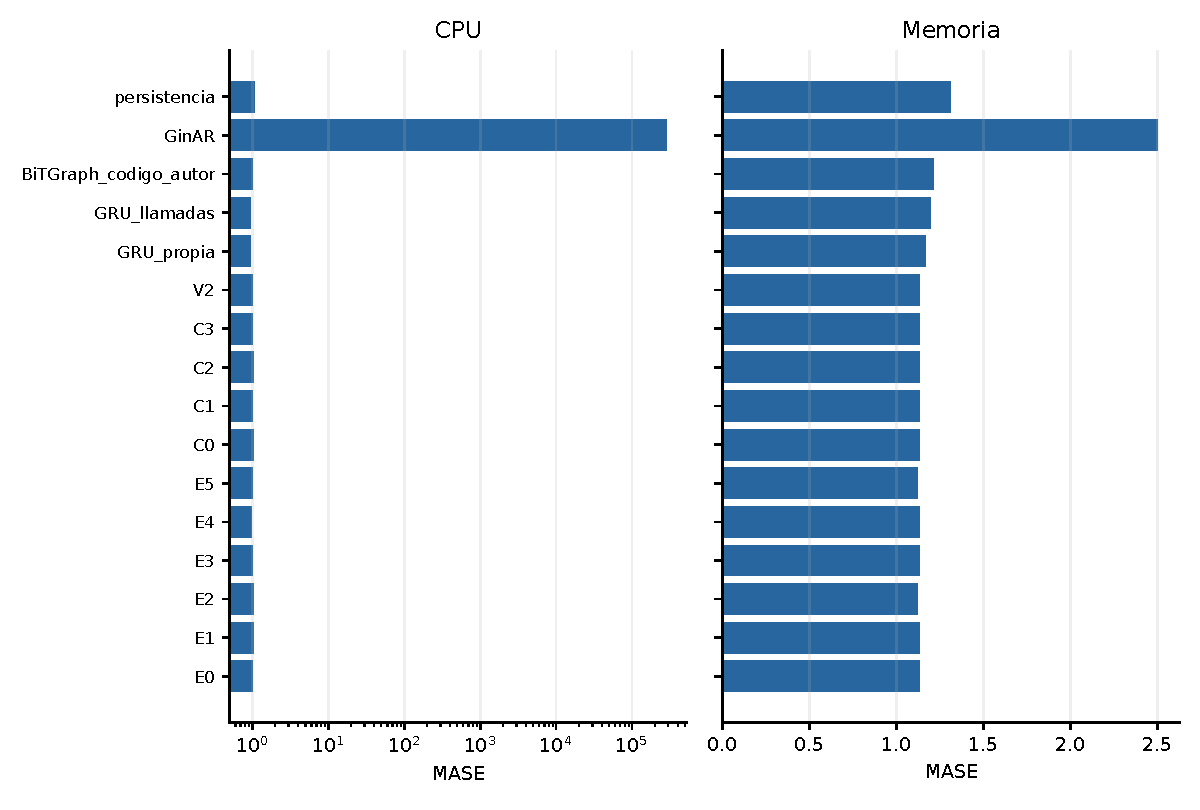
\includegraphics[width=0.82\textwidth]{figuras/es_historico.pdf}
\caption{MASE histórico de seis condiciones con pérdidas. La escala logarítmica CPU conserva el extremo de GinAR; memoria utiliza escala lineal. Son resultados fuente 28.}\label{fig:historical}\end{figure*}
\begin{figure*}[!t]\centering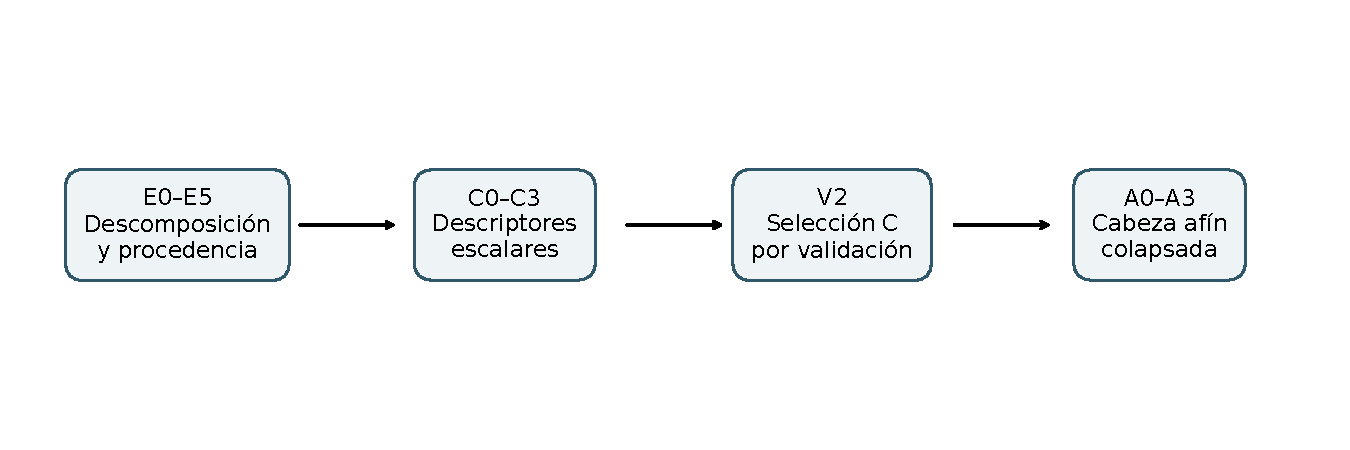
\includegraphics[width=0.91\textwidth]{figuras/es_evolucion.pdf}
\caption{E cambia descomposición o descriptores completos; C mantiene dos cabezas con descriptores escalares; V2 selecciona ajustes C existentes; A colapsa la proyección afín fija. Las flechas indican orden de estudio, sin garantizar mejoras.}\label{fig:evolution}\end{figure*}

\subsection{Finalización ampliada, integridad y pérdidas realizadas}\label{sec:completion}
Se completaron L12/H1, seis configuraciones secundarias y transferencia externa con pesos congelados:364 ajustes neuronales finales, 56 registros simples por configuración/recurso y 280 ajustes cortos fuente. Se guardaron 9680 archivos de predicciones y 3097600 filas de métricas por servicio. La reconstrucción independiente float 64 comprobó índices, cantidades de objetivos, resúmenes criptográficos y MAE/RMSE/MASE desde todos los archivos. La discrepancia absoluta máxima fue $3.73\times 10^{-9}$ en unidades originales. Los 420 checkpoints finales y hashes fuente pasaron la auditoría. Las filas reiteran modelos, máscaras, semillas, servicios y condiciones; no representan datasets independientes.

Con etiqueta 20\%, los cuatro mecanismos de conteo exacto produjeron 19.988\% de ausencia inducida en la prueba ChronoGraph. MAR dependiente del retardo promedió 26.301\%, con rango 25.925--26.577\% entre veinte máscaras. En Alibaba el redondeo dio 20.833\% para conteo exacto y MAR 27.861\%, rango 26.042--30.469\%. La ausencia natural se registra aparte. El corte 70/10/20 corresponde a filas ChronoGraph; Alibaba contiene 12 intervalos de calibración y 36 objetivos.

\subsection{Comparación principal sobre 32 servicios}
La Tabla~\ref{tab:primary} y la Fig.~\ref{fig:models} presentan L12/H1 y seis condiciones originales con pérdidas. PatchTST tuvo los menores promedios MASE observados:1.0419 CPU y 1.2170 memoria; NLinear quedó cerca con 1.0463 y 1.2197. No se preespecificó una prueba confirmatoria entre ambos. La media móvil obtuvo CPU 1.0678, menor que DLinear 1.1493, E5 1.1454 y A3 1.1602. En memoria A0 fue la menor variante afín compacta, 1.2334; A3 obtuvo 1.2403, DLinear 1.2402 y E5 1.2656. Los dos coeficientes de ausencia no mejoraron el agregado A3 frente a A0. El beneficio histórico de E5 en memoria no se conservó como victoria sobre DLinear. GRU de grafo alcanzó memoria 1.4851; ninguna familia se eliminó por mal resultado.
\begin{table*}[!t]
\caption{Principal destino 32: ponderación igual de servicios, seis condiciones con pérdidas, máscaras y ajustes. MAE/RMSE CPU se muestran en $10^{-3}$ de escala publicada y memoria en MiB,$2^{20}$ bytes. MASE es adimensional. El rango no constituye significación.}\label{tab:primary}
\centering\footnotesize
\FitTable{\begin{tabular}{lrrrrrr}
\toprule
Modelo & CPU MASE & CPU MAE & CPU RMSE & Mem. MASE & Mem. MAE & Mem. RMSE \\
\midrule
Persistencia & 1.1170 & 3.3236 & 4.5878 & 1.2861 & 2.0009 & 3.3833 \\
Media móvil & 1.0678 & 2.9643 & 4.2038 & 1.2361 & 1.8956 & 3.2699 \\
Suavizamiento exponencial & 1.0691 & 2.8926 & 4.0646 & 1.2535 & 1.9130 & 3.2673 \\
Ridge & 1.2669 & 3.1952 & 4.3079 & 1.3613 & 1.9589 & 3.1848 \\
DLinear & 1.1493 & 2.9924 & 4.1015 & 1.2402 & 1.8762 & 3.1573 \\
NLinear & 1.0463 & 2.8499 & 3.9969 & 1.2197 & 1.8482 & 3.1422 \\
E5 & 1.1454 & 3.0142 & 4.1411 & 1.2656 & 1.9044 & 3.1560 \\
A0 & 1.1562 & 3.0028 & 4.1185 & 1.2334 & 1.8649 & 3.1605 \\
A1 & 1.1547 & 2.9986 & 4.1147 & 1.2397 & 1.8704 & 3.1591 \\
A2 & 1.1563 & 3.0030 & 4.1185 & 1.2443 & 1.8773 & 3.1650 \\
A3 & 1.1602 & 3.0095 & 4.1248 & 1.2403 & 1.8733 & 3.1629 \\
GRU (propia) & 1.2198 & 3.2253 & 4.5667 & 1.3438 & 2.1652 & 3.7094 \\
GRU (grafo) & 1.1949 & 3.2375 & 4.5153 & 1.4851 & 2.2017 & 3.6563 \\
GRU-D adaptada & 1.1766 & 3.1392 & 4.4427 & 1.3605 & 2.1647 & 3.6811 \\
PatchTST (pequeño) & 1.0419 & 2.8539 & 4.1061 & 1.2170 & 1.8649 & 3.1655 \\
\bottomrule
\end{tabular}
}
\end{table*}
\begin{figure*}[!t]\centering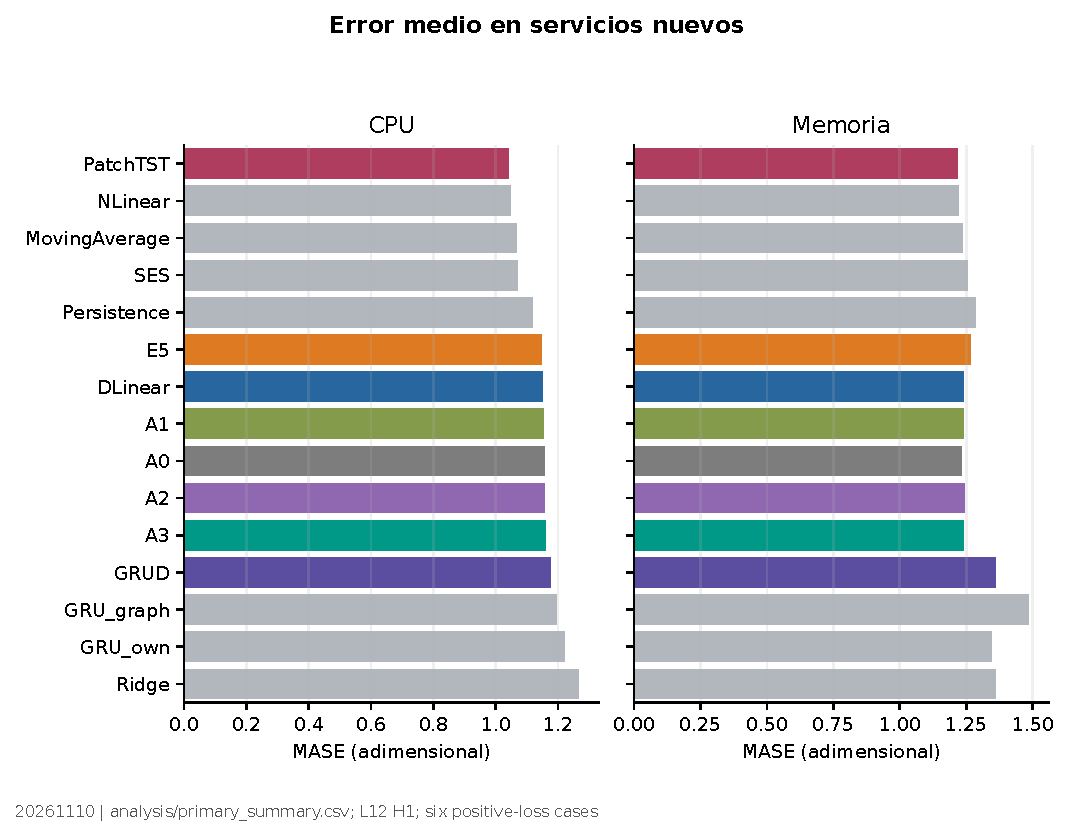
\includegraphics[width=0.79\textwidth]{figuras/es_06_models.pdf}
\caption{MASE principal de quince familias. La ordenación CPU solo organiza la presentación. Comparten servicios, máscaras y objetivos; se conserva la variación entre ajustes neuronales.}\label{fig:models}\end{figure*}

\subsection{Cuatro contrastes preespecificados y evaluación de A3}\label{sec:contrasts}
La Tabla~\ref{tab:contrasts} distingue diferencia media MASE y reducción media por celda. El único contraste con diez de diez semillas favorables fue A3 contra E5 en memoria:$\Delta=0.02523$, prueba bilateral exacta de signos ajustada Holm $ p=0.0078125$, intervalo condicional cruzado con bloques 48$[0.01312,\allowbreak 0.03981]$. La reducción media emparejada por celda fue 1.00\%; el cociente de medias da 1.99\%, otro estimando. Excluir la semilla de búsqueda 101 dejó nueve de nueve favorables y $ p=0.015625$ diagnóstico ajustado separadamente. Estos valores están condicionados a servicios, máscaras y período fijos, sin demostrar mejora de una población de sistemas.

Frente a DLinear, A3 tuvo $\Delta=-0.01090$ en CPU y $-0.00014$ en memoria, ambos $ p $ ajustada 1. Contra E5 en CPU,$\Delta=-0.01485$ y $ p=1$. Su intervalo temporal condicional excluye cero hacia valores negativos, mientras solo tres de diez semillas favorecen A3 y la prueba principal no rechaza. Los procedimientos tienen estimandos y supuestos diferentes; el intervalo no reemplaza la regla de cuatro pruebas. La Tabla~\ref{tab:block} presenta sensibilidad a bloques de 24, 48 y 96 pasos.
\begin{table*}[!t]
\caption{Contrastes principales:$\Delta=MASE_{referencia}-MASE_{A3}$. Positivo favorece A3. La media $ R $ promedia porcentajes de celdas, no cocientes globales. Los intervalos condicionan servicios fijos; las pruebas usan dirección de medias por semilla y Holm.}\label{tab:contrasts}
\centering\footnotesize
\FitTable{\begin{tabular}{lrrrrrr}
\toprule
Recurso & Referencia & $\Delta$MASE & Media $R$ (\%) & Condicional95\% interval & $p_{\mathrm{Holm}}$ & Semillas favorables \\
\midrule
CPU & DLinear & -0.01090 & -0.78 & [-0.02732, 0.00470] & 1 & 4/10 \\
CPU & E5 & -0.01485 & -1.95 & [-0.02977, -0.00120] & 1 & 3/10 \\
Memoria & DLinear & -0.00014 & 0.00 & [-0.00959, 0.01035] & 1 & 3/10 \\
Memoria & E5 & 0.02523 & 1.00 & [0.01312, 0.03981] & 0.007812 & 10/10 \\
\bottomrule
\end{tabular}
}
\end{table*}

La ventaja de memoria frente a E5 es heterogénea: favorece solo 10 de 32 servicios; service 540 aporta 42.4\% de la media. Excluirlo después de observar resultados deja $\Delta=0.01499$; excluir los tres servicios más favorables deja 0.00325 y seis de diez semillas favorables. Son exclusiones informadas por resultados, no análisis confirmatorios. La Fig.~\ref{fig:services} muestra los efectos por servicio predefinidos frente a DLinear. La Fig.~\ref{fig:ablation} conserva A0--A3 y la Fig.~\ref{fig:seeds} separa ajustes. Las máscaras repiten evaluación de los mismos pesos; no añaden entrenamientos independientes.
\begin{figure*}[!t]\centering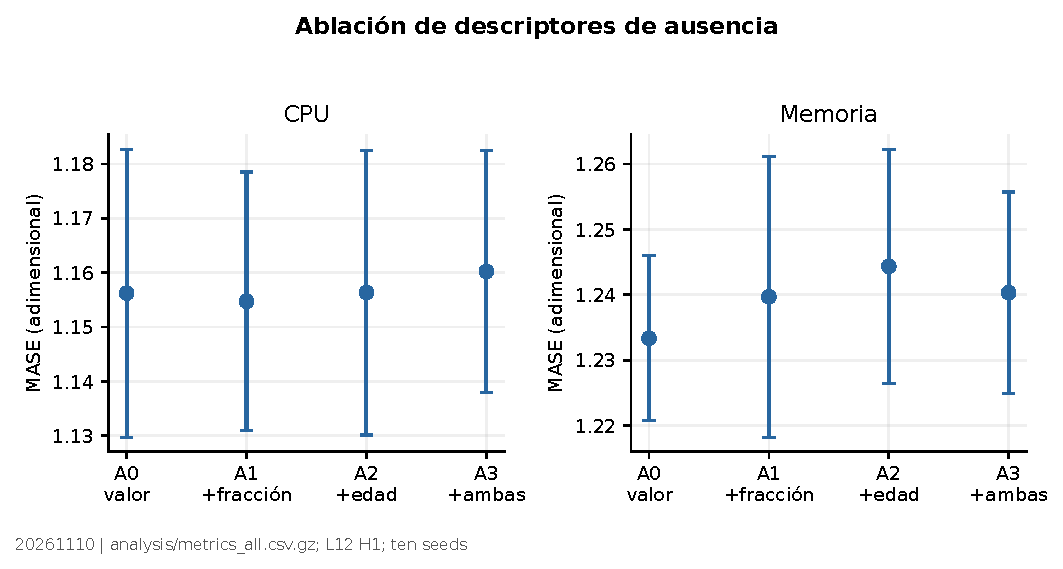
\includegraphics[width=0.79\textwidth]{figuras/es_11_ablations.pdf}
\caption{Medias A0--A3 y desviaciones entre diez medias de ajustes. Las barras son desviaciones descriptivas, no intervalos de confianza ni predictivos. Las familias se seleccionaron independientemente.}\label{fig:ablation}\end{figure*}
\begin{figure*}[!t]\centering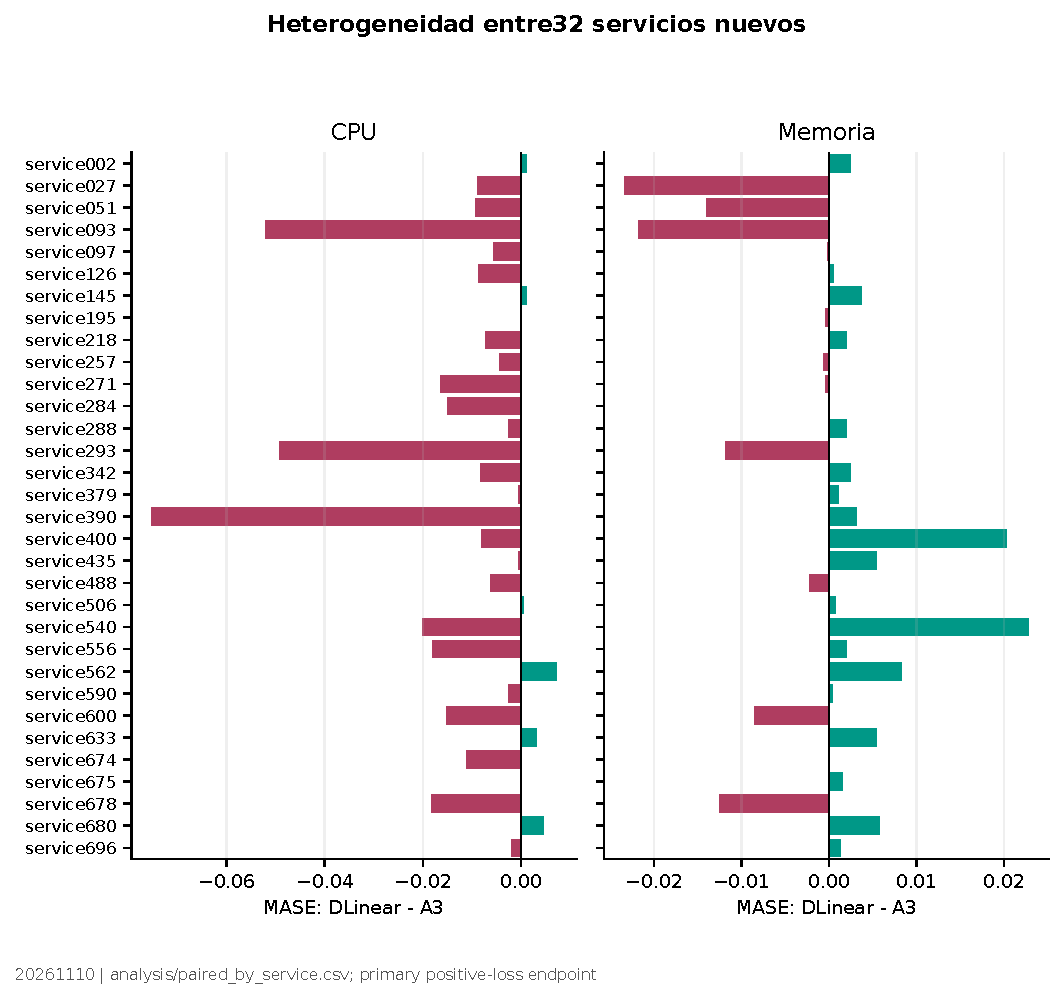
\includegraphics[width=0.71\textwidth]{figuras/es_15_services.pdf}
\caption{DLinear menos A3 por servicio, promediando semillas, máscaras y seis condiciones. Positivo favorece A3. Los servicios conectados son casos fijos, no muestras poblacionales independientes.}\label{fig:services}\end{figure*}
\begin{figure*}[!t]\centering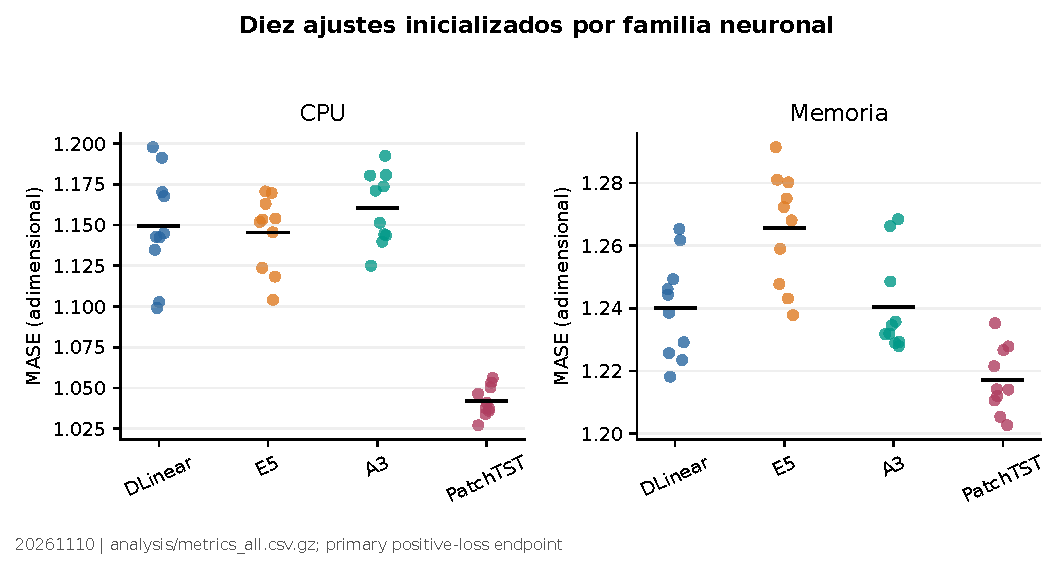
\includegraphics[width=0.76\textwidth]{figuras/es_10_seed_variability.pdf}
\caption{Diez medias por ajuste neuronal sobre servicios fijos, seis condiciones y veinte máscaras. Las marcas negras indican promedio; no son diez infraestructuras.}\label{fig:seeds}\end{figure*}

\subsection{Robustez frente a telemetría incompleta}
Las curvas de medias generalmente aumentan entre datos completos y 40\% de ausencia dispersa o por bloques cortos, Fig.~\ref{fig:loss}. No se afirma monotonía para cada servicio o máscara. A etiqueta 20\%, bloques prolongados fueron más difíciles que pérdidas correlacionadas para A3: CPU 1.2330 frente a 1.1342 y memoria 1.3743 frente a 1.1932. MAR no es una comparación controlada a 20\% porque realiza una fracción mayor. El suplemento retiene los tres mecanismos y todas las familias. Los ejemplos de máscaras muestran estructura espacial y duración impuestas, no fallas reales. Seleccionar una curva favorable no determina la conclusión.
\begin{figure*}[!t]\centering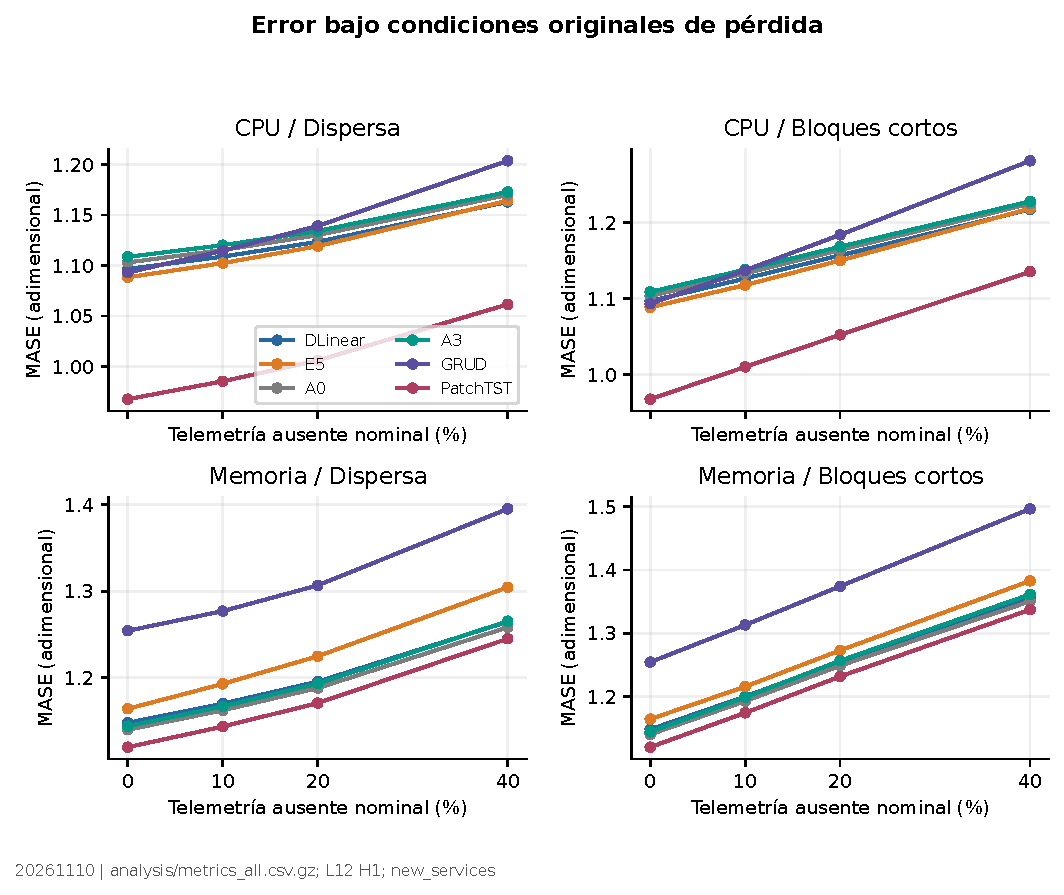
\includegraphics[width=0.76\textwidth]{figuras/es_07_loss.pdf}
\caption{MASE descriptivo bajo datos completos y pérdidas originales dispersas o por bloques. Las curvas seleccionadas facilitan lectura; las tablas y CSV conservan toda la comparación.}\label{fig:loss}\end{figure*}

\subsection{Horizontes directos y ventanas}
La comparación secundaria utiliza 1553 objetivos destino idénticos, filas 6452--8004, tres semillas, cinco máscaras y seis condiciones con pérdidas. A L12, CPU PatchTST aumenta de 1.0445 a treinta minutos a 1.6399 a seis horas; A3 pasa de 1.1584 a 1.9779. En memoria PatchTST pasa de 1.2264 a 2.1681 y A3 de 1.2436 a 2.3141. Cada horizonte ajusta un modelo directo; no son predicciones iteradas de un paso. Las historias más largas producen resultados mixtos: CPU A3 mejora de 1.1584 en L12 a 1.0966 en L48, pero memoria empeora de 1.2436 a 1.2560. PatchTST memoria tiene su menor valor de las tres historias en L24, 1.2190.

El punto H30 común difiere deliberadamente del principal completo y no lo sustituye. Las Figs.~\ref{fig:horizon} y~\ref{fig:history} y las Tablas~\ref{tab:horizon} y~\ref{tab:history} conservan el diseño estrella; no se ejecutaron todas las combinaciones de ventanas y horizontes. Una curva une observaciones ejecutadas sin demostrar interacciones factoriales ni significación confirmatoria.
\begin{figure*}[!t]\centering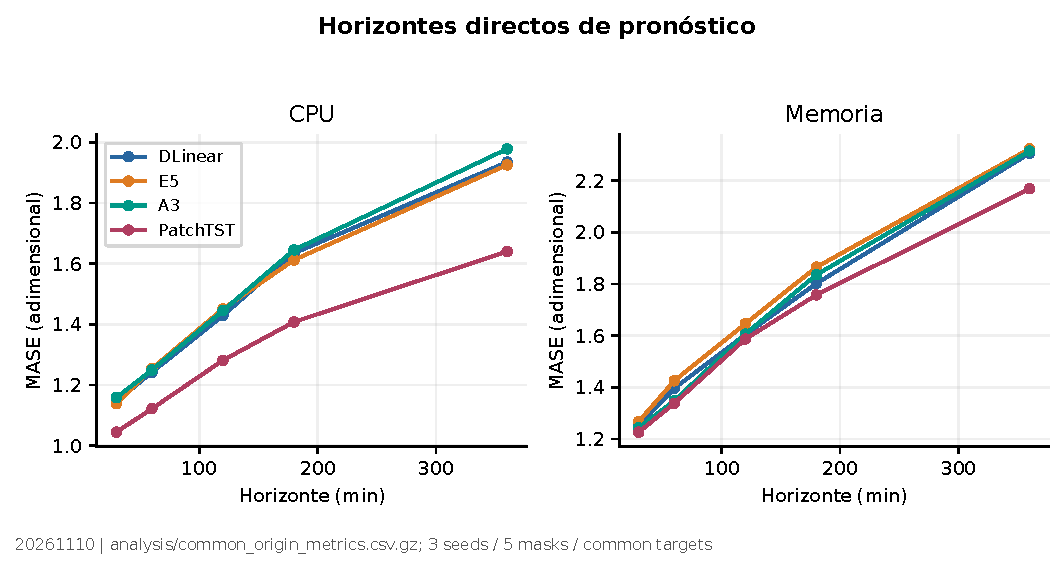
\includegraphics[width=0.79\textwidth]{figuras/es_08_horizon.pdf}
\caption{MASE con horizontes directos sobre 1553 objetivos comunes, tres semillas y cinco máscaras. Cada extremo usa pesos ajustados para ese horizonte.}\label{fig:horizon}\end{figure*}
\begin{figure*}[!t]\centering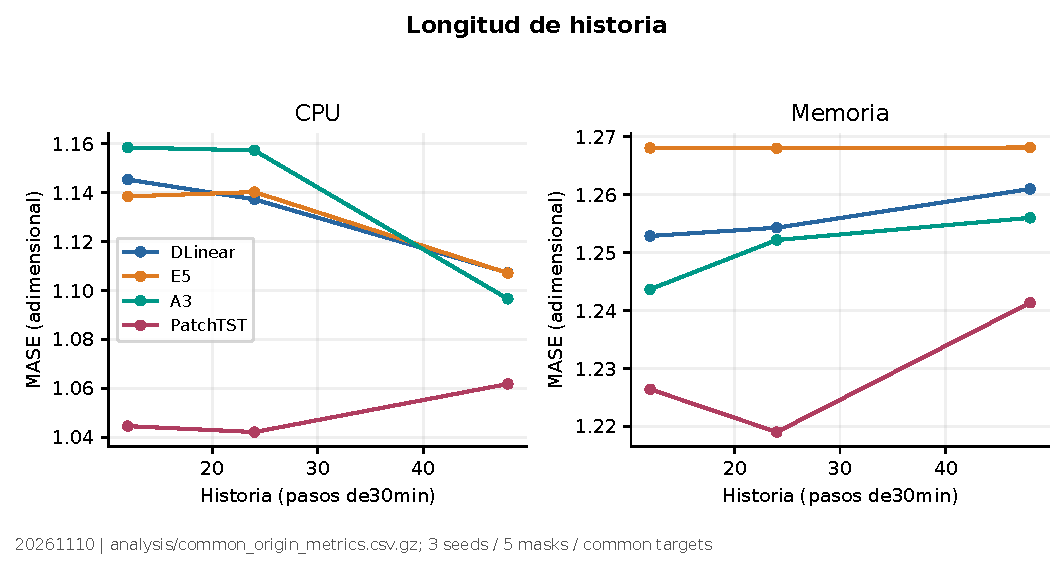
\includegraphics[width=0.79\textwidth]{figuras/es_09_history.pdf}
\caption{Sensibilidad a historia con horizonte treinta minutos y mismo soporte secundario. Las líneas son descriptivas.}\label{fig:history}\end{figure*}

\subsection{Transferencia externa a Alibaba}
En el día Alibaba, persistencia obtuvo el menor MASE de las catorce familias elegibles:2.3795 en CPU y 7.5150 en memoria normalizadas. A3 obtuvo 3.3593 y 9.9535; PatchTST 3.1112 y 10.5876. No se reajustó ningún método sobre los 36 intervalos objetivo. GRU de grafo se excluyó por ausencia de red externa. El denominador de seis horas y la diferencia entre medias de intervalos y muestras puntuales limitan la interpretación. Los errores absolutos de la Tabla~\ref{tab:external} son utilización normalizada, sin comparación directa con bytes o escala CPU ChronoGraph.

La Fig.~\ref{fig:external} conserva la inversión de clasificación: la mejor media primaria no se convierte en una ventaja universal entre dominios. Un día, 32 servicios elegidos por disponibilidad y 36 objetivos por servicio no sustentan validación externa concluyente. El volumen bruto de cientos de millones de filas documenta procesamiento, no tamaño efectivo independiente de evaluación.
\begin{figure*}[!t]\centering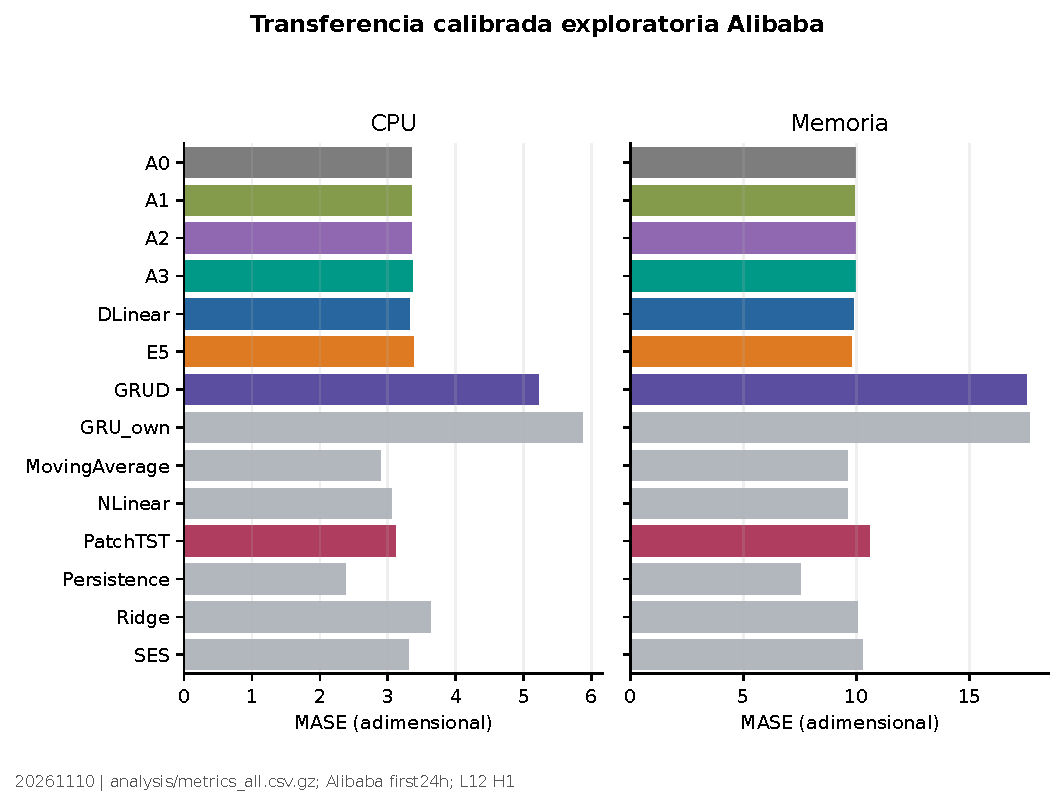
\includegraphics[width=0.79\textwidth]{figuras/es_12_external.pdf}
\caption{Transferencia exploratoria del primer día Alibaba:32 servicios, 36 objetivos semihorarios y seis horas de calibración. No representa replicación independiente entre infraestructuras.}\label{fig:external}\end{figure*}

\subsection{Coste computacional}\label{sec:cost}
A L12, A3 tiene 15 parámetros por recurso, DLinear 26 y E5 74. En B1/32 servicios, p 50 CPU fue 0.050~ms para A3, 0.057 para DLinear y 0.295 para E5; CUDA sincronizada 0.141, 0.281 y 0.665~ms. PatchTST tiene 2499 elementos entrenables y p 50 CPU 0.521~ms/CUDA1.212~ms. La Tabla~\ref{tab:efficiency} conserva p 95 y todas las familias. Son llamadas con tensores residentes, sin recolección, preparación o control. Algunos modelos compactos resultan más lentos en CUDA que CPU con este lote pequeño.

Las medianas de sumas de épocas completadas, incluyendo validación, fueron 8.56~s A3, 10.21 DLinear, 14.72 E5 y 42.88 PatchTST. Excluyen búsqueda, escritura de checkpoints e intentos incompletos fallidos. La Fig.~\ref{fig:latency} relaciona error con p 50 y la Fig.~\ref{fig:params} con tamaño. Las diferencias observadas no identifican una aceleración causal universal de hardware ni beneficios de SLA.
\begin{table*}[!t]
\caption{Elementos entrenables y p 50/p 95 en ms, B1/32 servicios. CUDA sincroniza ensayos y GRU-D usa reproducción sin coste inicial de captura. La suma de épocas es mediana de ajustes fuente, no duración total del proyecto.}\label{tab:efficiency}
\centering\footnotesize
\FitTable{\begin{tabular}{lrrrrrr}
\toprule
Modelo & Parámetros & CPU p50 & CPU p95 & CUDA p50 & CUDA p95 & Suma de épocas (s) \\
\midrule
Persistencia & 0 & 0.005 & 0.005 & 0.012 & 0.012 & sin medir \\
Media móvil & 0 & 0.014 & 0.015 & 0.023 & 0.025 & sin medir \\
Suavizamiento exponencial & 0 & 0.195 & 0.417 & 0.328 & 0.337 & sin medir \\
Ridge & 13 & 0.022 & 0.024 & 0.084 & 0.092 & sin medir \\
DLinear & 26 & 0.057 & 0.064 & 0.281 & 0.337 & 10.21 \\
NLinear & 13 & 0.031 & 0.045 & 0.095 & 0.102 & 7.62 \\
E5 & 74 & 0.295 & 0.317 & 0.665 & 0.681 & 14.72 \\
A0 & 13 & 0.022 & 0.023 & 0.085 & 0.095 & 7.26 \\
A1 & 14 & 0.046 & 0.049 & 0.125 & 0.134 & 7.99 \\
A2 & 14 & 0.030 & 0.032 & 0.104 & 0.116 & 7.10 \\
A3 & 15 & 0.050 & 0.056 & 0.141 & 0.166 & 8.56 \\
GRU (propia) & 841 & 0.425 & 0.450 & 0.341 & 0.360 & 15.41 \\
GRU (grafo) & 841 & 0.413 & 0.439 & 0.344 & 0.352 & 15.60 \\
GRU-D adaptada & 615 & 1.475 & 2.789 & 0.443 & 0.444 & 15.72 \\
PatchTST (pequeño) & 2499 & 0.521 & 0.546 & 1.212 & 1.316 & 42.88 \\
\bottomrule
\end{tabular}
}
\end{table*}
\begin{figure*}[!t]\centering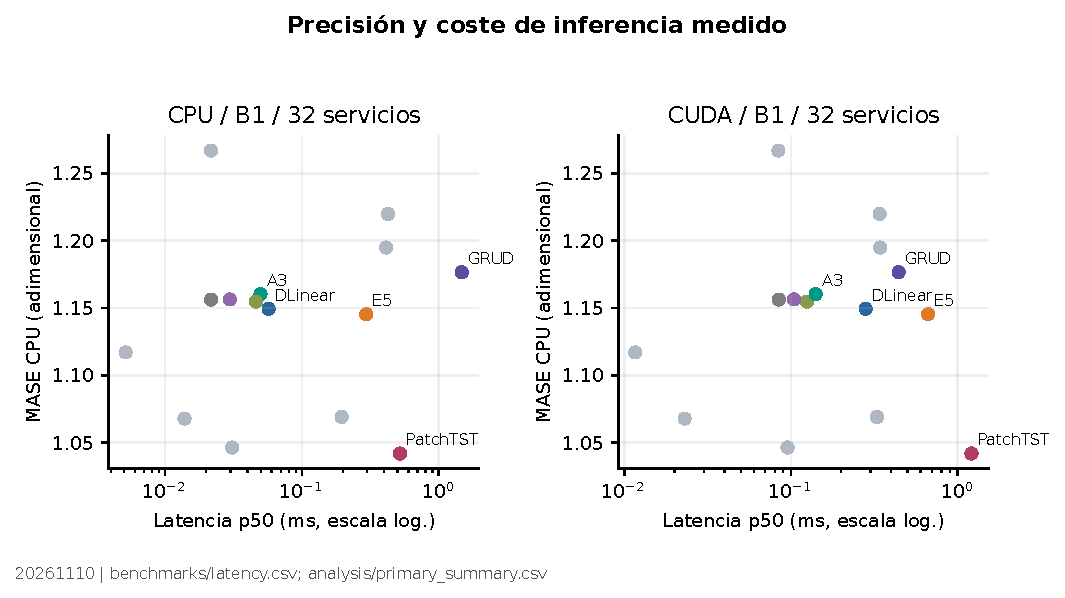
\includegraphics[width=0.79\textwidth]{figuras/es_13_latency.pdf}
\caption{MASE CPU y p 50 con entradas residentes. El equipo compartido y el alcance de la llamada limitan la interpretación operativa.}\label{fig:latency}\end{figure*}
\begin{figure*}[!t]\centering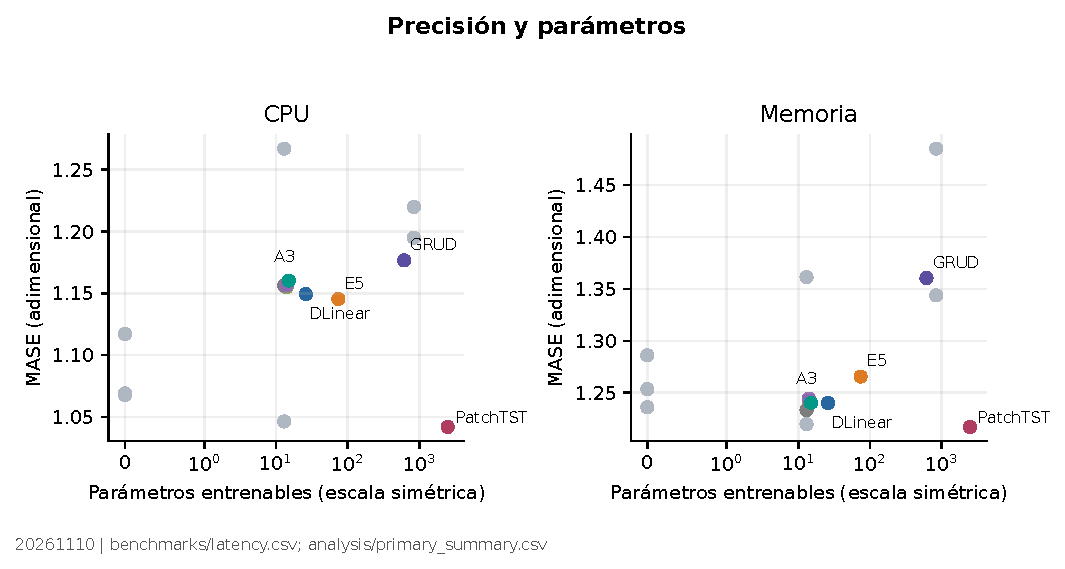
\includegraphics[width=0.79\textwidth]{figuras/es_14_parameters.pdf}
\caption{Error frente a parámetros entrenables. La escala logarítmica simétrica conserva referencias de cero parámetros. No incluye estados, calibración o coordinación.}\label{fig:params}\end{figure*}

El monitor muestreó RSS máximo del proceso 1725.47~MiB, sin capturar continuamente el pico. La RAM disponible del sistema se mantuvo sobre 10.87~GiB. La memoria GPU total alcanzó 3536~MiB y temperatura 75 gradosC; incluyen otras aplicaciones. El sensor CPU llegó a 92 gradosC y hubo un episodio de pausa del guardián. Se preservaron siete intentos GRU-D fallidos iniciales, 22 reintentos de entrenamiento por falta de memoria y 94 reducciones de lote de inferencia; todas las configuraciones finales tienen marcadores completos. No se midió energía del proyecto.

\subsection{Respuestas integradas a las preguntas}
La Tabla~\ref{tab:rq} conecta las fases sin promediar evidencia incompatible. La mejora histórica de memoria motiva una pregunta, sin sumarse a la ampliada para producir un efecto mayor. El volumen Alibaba no sustituye sus 36 objetivos. La auditoría verifica consistencia entre predicciones y métricas, no independencia de todo preprocesamiento desconocido del proveedor.
\begin{table*}[!t]
\caption{Respuestas basadas en evidencia. Las direcciones corresponden al experimento indicado y las cuatro pruebas principales se presentan por separado.}\label{tab:rq}
\centering\footnotesize
\begin{tabularx}{\linewidth}{p{.07\linewidth}XXX}
\toprule PI & Evidencia y dirección & Alcance & Límite \\\midrule
1 & Pérdidas originales elevan generalmente medias; bloques largos empeoran A3 & Trazas y mecanismos sintéticos & No prueba fallas reales ni todos los servicios \\
2 & E5 histórico mejora memoria y empeora CPU; DLinear fijo es afín & Parametrizaciones E/C/A separadas & Selección y optimización diferentes \\
3 & A3 no supera A0 agregado; descriptores E mixtos & Familias seleccionadas independientemente & No efecto causal ortogonal \\
4 & A3 usa 15 frente a 26/74; menor latencia medida & B1 residente CPU/CUDA medidos & Sin ventaja universal de precisión o energía \\
5 & PatchTST/NLinear menores medias principales; persistencia menor MASE externo & Destino 32 calibrado y un día Alibaba & Sin período independiente o validación poblacional \\
6 & Intervalos históricos cruzados amplios;A3/E5 memoria 10/10 & Datos y configuraciones fijos & Concentración por servicio y dependencia temporal \\
\bottomrule\end{tabularx}
\end{table*}

\section{Discusión}\label{sec:discussion}
A3 demuestra reducción de parámetros y una ventaja observada de memoria frente a E5 sobre los servicios nuevos fijos. La evidencia completa no respalda mejora uniforme. CPU A3 empeora frente a ambas referencias principales, A0 tiene menor memoria MASE que A3 y PatchTST pequeño obtiene la menor media principal. La ventaja contra E5 se concentra en una minoría de servicios, aunque la dirección por semilla es consistente bajo la comparación preespecificada. Las exclusiones posteriores informadas por resultados explican por qué esa consistencia no equivale a portabilidad espacial amplia.

El resultado algebraico delimita la aportación: dos cabezas afines tras un filtro móvil fijo siguen siendo una función afín. Reducir parámetros puede bajar el coste de ejecución medido, pero cambia la trayectoria de Adam y la interacción con regularización. Los coeficientes de ausencia pueden mejorar o empeorar. EMA dependiente de disponibilidad en E5 no queda incluida en ese colapso. Las medias A1/A2/A3 seleccionadas independientemente no prueban un beneficio aditivo general. Un estudio mecanístico posterior podría fijar hiperparámetros, igualar regularización y evaluar interacciones sobre otro período independiente; son propuestas, no experimentos ejecutados.

La transición histórica-ampliada modifica más que las semillas. Los servicios destino tienen distinta calibración, otro papel en el ajuste y una receta fuente con diez condiciones. El cambio de rango de E5 no puede atribuirse únicamente a aumentar servicios o inicializaciones. La mejora histórica de memoria, su conservación incompleta por C/V2 y el contraste A3 posterior responden conjuntamente a la parsimonia: reducir coeficientes puede mantener un error observado aceptable y perder una ventaja previa específica. Una comparación favorable posterior tampoco restablece superioridad universal.

NLinear y PatchTST sugieren competitividad de un nivel reciente explícito y una representación por parches bajo transferencia fuente. No se aíslan esos mecanismos: cambian configuraciones, parametrización y, en PatchTST, atención y normalización. NLinear tiene MAE CPU mostrado ligeramente menor que PatchTST pese al orden contrario de MASE. MASE pondera respecto de variación histórica por servicio; el error absoluto conserva la unidad física. La clasificación depende de la función de pérdida y la cohorte, sin que una métrica invalide automáticamente a la otra.

Los horizontes directos mayores aumentan errores mostrados de los modelos seleccionados, pero utilizan pesos propios y objetivos comunes; no prueban acumulación recursiva. Las historias largas producen mejora CPU y empeoramiento memoria en A3. Contener más valores aumenta coeficientes, procesamiento y exposición potencial a regímenes antiguos; no garantiza generalización. El diseño estrella describe elecciones concretas, sin estimar todas las interacciones ventana-horizonte.

El caso externo cambia dominio y definición de medición. La ventaja de persistencia es compatible con una traza corta de utilización normalizada relativamente estable, pero no establece su causa. No hubo grafo externo y seis horas pueden producir denominadores pequeños. Se muestran MASE y errores absolutos normalizados juntos, sin combinar magnitudes con errores físicos ChronoGraph. Más días, servicios elegidos independientemente y datasets con preparación documentada permitirían estudiar estabilidad de rangos.

La eficiencia ofrece una perspectiva acotada. A3 es menor que E5 y tiene menor p 50 con tensores residentes en ambos dispositivos. PatchTST presenta menor MASE principal con mayor coste medido; media móvil resulta una referencia CPU fuerte sin pesos entrenables. En lotes pequeños, lanzamiento y sincronización pueden favorecer CPU frente a CUDA. No se demuestra menor energía, recolección más rápida o mejor autoescalado. Evaluarlo exigiría controlador, reproducción de cargas, tiempos completos, métricas SLA e instrumentación energética atribuible al proyecto.

La corrección histórica de unidades de intervalos es sustantiva: un intervalo absoluto MASE no puede leerse como porcentaje porque aparezca junto a una reducción porcentual. En la ampliación, porcentajes por celda y cociente de medias se mantienen separados. La prueba de signos mide consistencia de dirección entre ajustes y el intervalo por bloques aproxima una media remuestreada. Su desacuerdo es posible sin error aritmético y no permite sustituir el criterio principal por el más favorable. Así se evita que un rango o una incertidumbre condicional estrecha se convierta en superioridad poblacional no demostrada.

El histórico conserva alcance distinto y genera hipótesis. La transferencia espacial cambia el orden y Alibaba lo cambia otra vez. El extremo GinAR se retiene como resultado de implementación/protocolo, sin refutar el método publicado. La contribución reproducible es documentar cuándo capacidad, procedencia de observaciones, error, coste y dominio dejan de coincidir en una misma recomendación.

La dinámica calculada solo en entrenamiento aporta contexto para interpretar los dos recursos. La autocorrelación mediana de primer retardo entre las 28 series es 0.447 en CPU y 0.867 en memoria. El cambio absoluto relativo a la desviación de cada serie tiene medianas 0.413 y 0.275. Son valores compatibles con mayor persistencia de nivel en memoria. No identifican la causa del cambio de error con EMA: el residual conserva las desviaciones del nivel y ambas cabezas se ajustan juntas. Motivan un análisis controlado alrededor de cambios abruptos, sin afirmar que suavizar retrasa mecánicamente el pronóstico final.

\section{Amenazas a la validez}
\paragraph{Validez de constructo.} El uso registrado no es demanda sin restricciones. Las muestras ChronoGraph y las medias Alibaba de intervalos completados tienen semánticas diferentes; la normalización externa no representa bytes o núcleos. Las ausencias sintéticas afectan entradas y dejan objetivos originales para evaluación, sin establecer incidencia o causa de averías reales. La calibración supone prefijos disponibles antes de degradación artificial. Arrastre y edad retienen información anterior a la ventana nominal.

\paragraph{Validez interna.} Estadísticas de prefijo, comprobaciones de partición/huecos, perturbación futura MAR, perturbación de valores ocultos con máscara fija y auditoría de predicciones abordan riesgos identificables. No certifican todo el procesamiento del proveedor. El alcance min--max externo y las fechas de disponibilidad de aristas permanecen inciertos. La validación fuente selecciona hiperparámetros y parada; el destino calibra sin ajustar pesos. Búsqueda estrecha, rotación de condiciones neuronales, ajuste analítico completo de ridge, parametrizaciones diferentes y BatchNorm por microlotes limitan igualdad de oportunidad de optimización. Las enmiendas de memoria y fallos recuperados se conservan.

\paragraph{Validez estadística.} Servicios dependientes, ventanas solapadas y máscaras emparejadas impiden tratar filas como réplicas independientes. Las semillas describen aleatoriedad algorítmica sobre datos fijos. La prueba exacta analiza dirección; la media de diferencias es otro efecto. Reutilizar 101 en selección se estudia solo mediante sensibilidad exploratoria. El bootstrap por bloques requiere aproximación local de dependencia; cambiar 24/48/96 no demuestra estacionariedad universal. Solo cuatro pruebas reciben control principal de multiplicidad. Los demás patrones, horizontes y cohortes son descriptivos.

\paragraph{Validez externa y sesgo histórico.} Fuente y destino ChronoGraph comparten infraestructura y período; la prueba fuente fue inspeccionada históricamente y parte de la prueba actual estuvo expuesta en validaciones anteriores. La selección topológica no es aleatoria. Un protocolo local fechado y exclusión de artefactos localizados no establecen cegamiento externo. Alibaba aporta un día, seis horas de calibración y 36 objetivos para 32 servicios seleccionados por disponibilidad. Sus millones de registros de pods no son millones de objetivos independientes. Normalización y agregación también cambian la tarea. Se requieren otros períodos, organizaciones y regímenes.

\paragraph{Eficiencia, hardware y validez operativa.} El portátil compartido introduce variación; una llamada con tensores residentes no mide desde el colector hasta el controlador. Lote, sincronización, captura e implementación afectan latencia. Los parámetros excluyen estados, preparación y coordinación. La memoria GPU del sistema incluye otras aplicaciones y RSS es muestreado, sin pico continuo. Las épocas excluyen costes de búsqueda y escritura; no identifican un efecto causal exclusivamente arquitectónico. No hay despliegue, controlador, medidor energético fiable ni beneficio SLA medido.

\paragraph{Reproducibilidad.} Los archivos permiten reconstruir cifras y comprobar pesos, pero la imagen derivada depende de una base local preservada. No se acredita una construcción limpia en otra máquina. Las verificaciones del mismo entorno no garantizan igualdad bit a bit entre versiones, dispositivos o kernels. El procesamiento del propietario y las licencias limitan lo que puede redistribuirse. Un repositorio público persistente y sus identificadores siguen pendientes, sin inventar disponibilidad o DOI.

\section{Conclusiones}
La representación de telemetría incompleta, la descomposición y la capacidad afectan de forma dependiente del recurso, escenario y selección. E5 histórico mejoró memoria 1.280\% y empeoró CPU 0.984\% en reducciones emparejadas; la variante compacta V2 no conservó toda la mejora. En 32 servicios adicionales, A3 redujo parámetros de 74 a 15 respecto de E5 y mejoró memoria MASE0.02523, con diez semillas favorables y $ p $ Holm 0.0078125. No superó a DLinear en la media principal y CPU empeoró frente a ambas referencias. La concentración en pocos servicios limita interpretar el efecto como mejora espacial general.

PatchTST pequeño tuvo las menores medias principales CPU/memoria, próximo a NLinear, sin prueba confirmatoria entre ambos. Las pérdidas y horizontes modificaron el error; ampliar historia produjo resultados mixtos. Persistencia obtuvo menor MASE en ambos recursos en el primer día Alibaba. Los resultados negativos y las referencias simples son parte de la respuesta científica, no excepciones que deban eliminarse. La reducción de tamaño tiene valor medido de inferencia, sin demostrar precisión universal ni ahorro operativo.

Los siguientes pasos son cohortes temporalmente independientes, períodos externos mayores, documentación de preparación y grafos, ausencias reales, intervenciones de componentes con regularización igualada y resultados de un controlador medidos. La reconstrucción local preserva cifras y límites. El uso editorial requiere aprobación de ambos autores, designación de correspondencia y decisiones sobre publicación previa y autorización de código/datos.

\section*{Disponibilidad de datos y código}
El código, las configuraciones y las métricas resumidas están disponibles en \href{https://github.com/Nunclear/prediccion-proactiva-de-recursos-computacionales-para-microservicios}{repositorio público del proyecto}. Las cohortes procesadas se distribuyen por separado para revisión académica. Los pesos, las predicciones y los objetos externos brutos se conservan en el archivo local de investigación. ChronoGraph y PatchTST conservan sus licencias de código; la invitación Alibaba al uso de investigación no establece por sí sola permiso ilimitado de redistribución. El uso y la difusión de datos deben respetar los términos de sus propietarios.
\section*{Contribuciones de los autores}
Las contribuciones individuales no han sido especificadas. No se infieren funciones CRediT ni ORCID. Ambos autores deben revisar el texto científico final y aprobar la versión de envío. El autor correspondiente continúa pendiente.
\section*{Financiación}
Esta investigación no recibió financiación externa.
\section*{Conflictos de interés}
Los autores declaran que no existen conflictos de interés.
\section*{Estado de versiones previas}
Los materiales locales acreditan un manuscrito histórico, pero no establecen si fue interno, entrega académica, prepublicación, enviado, aceptado o publicado. Los autores deben confirmarlo antes del envío. Una publicación o versión pública previa requiere cita y declaración de solapamiento pertinentes. No se infiere estado editorial a partir de un PDF local.

\FloatBarrier
\appendices
\section{Comparaciones detalladas suplementarias}
Las tablas conservan escenarios secundarios sin sustituir el criterio principal. La Tabla~\ref{tab:stress} contiene todas las familias bajo mecanismos añadidos; la Tabla~\ref{tab:variation} distingue variación de medias por semilla y por máscara. La desviación entre semillas no se define para una referencia determinista con un solo ajuste; no se sustituye silenciosamente por cero. Son resúmenes condicionados, no componentes independientes de varianza poblacional.
\begin{table*}[!t]
\caption{MASE descriptivo bajo pérdidas correlacionadas, prolongadas y MAR dependiente del retardo. La etiqueta nominal no equivale siempre a tasa realizada.}\label{tab:stress}
\centering\footnotesize
\FitTable{\begin{tabular}{lrrrrrr}
\toprule
Modelo & CPU corr. & CPU larga & CPU lag-MAR & Mem. corr. & Mem. larga & Mem. lag-MAR \\
\midrule
Persistencia & 1.0836 & 1.2113 & 1.0934 & 1.2422 & 1.4198 & 1.2493 \\
Media móvil & 1.0326 & 1.1509 & 1.0521 & 1.1885 & 1.3576 & 1.2091 \\
Suavizamiento exponencial & 1.0332 & 1.1470 & 1.0522 & 1.2024 & 1.3700 & 1.2254 \\
Ridge & 1.2453 & 1.3294 & 1.2518 & 1.3217 & 1.4826 & 1.3355 \\
DLinear & 1.1235 & 1.2222 & 1.1326 & 1.1956 & 1.3701 & 1.2120 \\
NLinear & 1.0121 & 1.1375 & 1.0281 & 1.1737 & 1.3532 & 1.1902 \\
E5 & 1.1194 & 1.2187 & 1.1300 & 1.2250 & 1.4072 & 1.2452 \\
A0 & 1.1300 & 1.2285 & 1.1393 & 1.1881 & 1.3638 & 1.2048 \\
A1 & 1.1285 & 1.2273 & 1.1377 & 1.1942 & 1.3701 & 1.2109 \\
A2 & 1.1299 & 1.2289 & 1.1393 & 1.1985 & 1.3783 & 1.2151 \\
A3 & 1.1342 & 1.2330 & 1.1428 & 1.1932 & 1.3743 & 1.2106 \\
GRU (propia) & 1.1879 & 1.3095 & 1.2019 & 1.2932 & 1.5458 & 1.3110 \\
GRU (grafo) & 1.1603 & 1.2816 & 1.1761 & 1.4235 & 1.7076 & 1.4393 \\
GRU-D adaptada & 1.1394 & 1.2605 & 1.1592 & 1.3076 & 1.5114 & 1.3286 \\
PatchTST (pequeño) & 1.0053 & 1.1323 & 1.0223 & 1.1712 & 1.3485 & 1.1894 \\
\bottomrule
\end{tabular}
}
\end{table*}
\begin{table*}[!t]
\caption{Desviaciones de medias por semilla y máscara, principal con pérdidas. No son incertidumbres de infraestructuras independientes.}\label{tab:variation}
\centering\footnotesize
\FitTable{\begin{tabular}{lrrrr}
\toprule
Modelo & CPU DE semilla & CPU DE máscara & Memoria DE semilla & Memoria DE máscara \\
\midrule
Persistencia & sin definir & 0.0033 & sin definir & 0.0065 \\
Media móvil & sin definir & 0.0031 & sin definir & 0.0062 \\
Suavizamiento exponencial & sin definir & 0.0034 & sin definir & 0.0082 \\
Ridge & sin definir & 0.0021 & sin definir & 0.0063 \\
DLinear & 0.0332 & 0.0023 & 0.0161 & 0.0062 \\
NLinear & 0.0081 & 0.0030 & 0.0112 & 0.0062 \\
E5 & 0.0227 & 0.0025 & 0.0179 & 0.0066 \\
A0 & 0.0265 & 0.0024 & 0.0126 & 0.0063 \\
A1 & 0.0238 & 0.0024 & 0.0215 & 0.0063 \\
A2 & 0.0262 & 0.0024 & 0.0179 & 0.0063 \\
A3 & 0.0222 & 0.0024 & 0.0154 & 0.0063 \\
GRU (propia) & 0.0634 & 0.0018 & 0.0341 & 0.0050 \\
GRU (grafo) & 0.0313 & 0.0022 & 0.0403 & 0.0051 \\
GRU-D adaptada & 0.0426 & 0.0020 & 0.0463 & 0.0050 \\
PatchTST (pequeño) & 0.0093 & 0.0030 & 0.0105 & 0.0062 \\
\bottomrule
\end{tabular}
}
\end{table*}
\begin{table}[!t]
\caption{Intervalos95\% cruzados por semilla, máscara y bloques circulares para referencia menos A3. Los bloques24/48/96 equivalen a12/24/48 horas nominales. No se afirma cobertura predictiva o poblacional.}\label{tab:block}
\centering\footnotesize
\FitTable{\begin{tabular}{lrrrr}
\toprule
Recurso & Referencia & Pasos del bloque & Inferior & Superior \\
\midrule
CPU & DLinear & 24 & -0.02818 & 0.00581 \\
CPU & DLinear & 48 & -0.02732 & 0.00470 \\
CPU & DLinear & 96 & -0.02944 & 0.00518 \\
CPU & E5 & 24 & -0.02903 & -0.00094 \\
CPU & E5 & 48 & -0.02977 & -0.00120 \\
CPU & E5 & 96 & -0.02966 & -0.00011 \\
Memoria & DLinear & 24 & -0.01024 & 0.01019 \\
Memoria & DLinear & 48 & -0.00959 & 0.01035 \\
Memoria & DLinear & 96 & -0.00988 & 0.00981 \\
Memoria & E5 & 24 & 0.01264 & 0.03961 \\
Memoria & E5 & 48 & 0.01312 & 0.03981 \\
Memoria & E5 & 96 & 0.01233 & 0.03971 \\
\bottomrule
\end{tabular}
}
\end{table}
\begin{table*}[!t]
\caption{MASE con objetivos comunes: CPU a la izquierda y memoria a la derecha, horizontes en minutos. Tres semillas, cinco máscaras y seis condiciones con pérdidas. H30 es un subconjunto del principal.}\label{tab:horizon}
\centering\footnotesize

\setlength{\tabcolsep}{4pt}
\begin{minipage}[t]{.485\textwidth}
\centering\FitTable{\begin{tabular}{lrrrrr}
\toprule
Modelo & 30 & 60 & 120 & 180 & 360 \\
\midrule
Persistencia & 1.1159 & 1.1381 & 1.3408 & 1.4851 & 1.7819 \\
Media móvil & 1.0666 & 1.1420 & 1.3589 & 1.4831 & 1.7010 \\
Suavizamiento exponencial & 1.0686 & 1.1469 & 1.3009 & 1.4242 & 1.6651 \\
Ridge & 1.2672 & 1.3856 & 1.6037 & 1.7441 & 2.0420 \\
DLinear & 1.1453 & 1.2419 & 1.4287 & 1.6340 & 1.9346 \\
E5 & 1.1384 & 1.2541 & 1.4506 & 1.6121 & 1.9251 \\
A3 & 1.1584 & 1.2492 & 1.4448 & 1.6451 & 1.9779 \\
PatchTST (pequeño) & 1.0445 & 1.1217 & 1.2814 & 1.4077 & 1.6399 \\
\bottomrule
\end{tabular}
}
\end{minipage}
\hfill
\begin{minipage}[t]{.485\textwidth}
\centering\FitTable{\begin{tabular}{lrrrrr}
\toprule
Modelo & 30 & 60 & 120 & 180 & 360 \\
\midrule
Persistencia & 1.2862 & 1.3398 & 1.6072 & 1.8097 & 2.2313 \\
Media móvil & 1.2364 & 1.3384 & 1.6286 & 1.7971 & 2.2460 \\
Suavizamiento exponencial & 1.2544 & 1.3549 & 1.5611 & 1.7315 & 2.1303 \\
Ridge & 1.3640 & 1.5179 & 1.8084 & 2.0411 & 2.5289 \\
DLinear & 1.2528 & 1.3958 & 1.6037 & 1.8014 & 2.3050 \\
E5 & 1.2680 & 1.4250 & 1.6459 & 1.8648 & 2.3222 \\
A3 & 1.2436 & 1.3474 & 1.6060 & 1.8353 & 2.3141 \\
PatchTST (pequeño) & 1.2264 & 1.3377 & 1.5866 & 1.7572 & 2.1681 \\
\bottomrule
\end{tabular}
}
\end{minipage}
\end{table*}
\begin{table*}[!t]
\caption{Historias semihorarias con objetivos comunes y horizonte treinta minutos (CPU a la izquierda y memoria a la derecha). Diseño estrella descriptivo.}\label{tab:history}
\centering\footnotesize

\setlength{\tabcolsep}{4pt}
\begin{minipage}[t]{.485\textwidth}
\centering\FitTable{\begin{tabular}{lrrr}
\toprule
Modelo & 12 & 24 & 48 \\
\midrule
Persistencia & 1.1159 & 1.1159 & 1.1159 \\
Media móvil & 1.0666 & 1.0666 & 1.0666 \\
Suavizamiento exponencial & 1.0686 & 1.0625 & 1.0618 \\
Ridge & 1.2672 & 1.2403 & 1.1504 \\
DLinear & 1.1453 & 1.1372 & 1.1072 \\
E5 & 1.1384 & 1.1402 & 1.1071 \\
A3 & 1.1584 & 1.1572 & 1.0966 \\
PatchTST (pequeño) & 1.0445 & 1.0421 & 1.0618 \\
\bottomrule
\end{tabular}
}
\end{minipage}
\hfill
\begin{minipage}[t]{.485\textwidth}
\centering\FitTable{\begin{tabular}{lrrr}
\toprule
Modelo & 12 & 24 & 48 \\
\midrule
Persistencia & 1.2862 & 1.2862 & 1.2862 \\
Media móvil & 1.2364 & 1.2364 & 1.2364 \\
Suavizamiento exponencial & 1.2544 & 1.2501 & 1.2494 \\
Ridge & 1.3640 & 1.3385 & 1.3063 \\
DLinear & 1.2528 & 1.2543 & 1.2610 \\
E5 & 1.2680 & 1.2680 & 1.2681 \\
A3 & 1.2436 & 1.2521 & 1.2560 \\
PatchTST (pequeño) & 1.2264 & 1.2190 & 1.2413 \\
\bottomrule
\end{tabular}
}
\end{minipage}
\end{table*}
\begin{table*}[!t]
\caption{Transferencia Alibaba, seis condiciones con pérdidas. MAE/RMSE absolutos utilizan normalización publicada de ambos recursos, no núcleos o bytes.}\label{tab:external}
\centering\footnotesize
\FitTable{\begin{tabular}{lrrrrrr}
\toprule
Modelo & CPU MASE & CPU MAE & CPU RMSE & Mem. MASE & Mem. MAE & Mem. RMSE \\
\midrule
Persistencia & 2.3795 & 0.007548 & 0.011324 & 7.5150 & 0.001085 & 0.002302 \\
Media móvil & 2.8906 & 0.009822 & 0.013787 & 9.6034 & 0.001392 & 0.002726 \\
Suavizamiento exponencial & 3.3095 & 0.011482 & 0.015495 & 10.2802 & 0.001847 & 0.003271 \\
Ridge & 3.6334 & 0.012690 & 0.016598 & 10.0263 & 0.001885 & 0.003208 \\
DLinear & 3.3262 & 0.011559 & 0.015422 & 9.8853 & 0.001762 & 0.003090 \\
NLinear & 3.0566 & 0.010455 & 0.014191 & 9.5989 & 0.001658 & 0.002972 \\
E5 & 3.3842 & 0.011791 & 0.015759 & 9.7985 & 0.001767 & 0.003104 \\
A0 & 3.3521 & 0.011664 & 0.015584 & 9.9413 & 0.001760 & 0.003097 \\
A1 & 3.3481 & 0.011650 & 0.015572 & 9.9291 & 0.001759 & 0.003095 \\
A2 & 3.3520 & 0.011663 & 0.015584 & 9.9668 & 0.001780 & 0.003117 \\
A3 & 3.3593 & 0.011686 & 0.015601 & 9.9535 & 0.001768 & 0.003105 \\
GRU (propia) & 5.8743 & 0.020136 & 0.024363 & 17.6403 & 0.004010 & 0.006199 \\
GRU-D adaptada & 5.2232 & 0.017836 & 0.022202 & 17.5279 & 0.003966 & 0.006144 \\
PatchTST (pequeño) & 3.1112 & 0.010653 & 0.015257 & 10.5876 & 0.001559 & 0.002796 \\
\bottomrule
\end{tabular}
}
\end{table*}
La Tabla~\ref{tab:historical} conserva los promedios históricos con telemetría completa incluida. La Tabla~\ref{tab:matrix} documenta el alcance de la ampliación y la repetición de filas de métricas.
\begin{table}[!t]
\caption{Resumen histórico de las siete condiciones originales, incluida telemetría completa. Su alcance difiere de la tabla histórica principal de seis condiciones con pérdidas. V2 es alias y el extremo GinAR se conserva.}\label{tab:historical}
\centering\footnotesize
\FitTable{\begin{tabular}{lrr}
\toprule
Modeloo histórico & CPU MASE & Memoria MASE \\
\midrule
persistencia & 1.0761 & 1.3112 \\
E0 & 0.9874 & 1.1283 \\
GRU\_propia & 0.9495 & 1.1580 \\
GRU\_llamadas & 0.9324 & 1.1893 \\
GinAR & 704115.0298 & 2.5812 \\
BiTGraph\_codigo\_autor & 0.9914 & 1.2009 \\
E1 & 1.0179 & 1.1283 \\
E2 & 1.0170 & 1.1178 \\
E3 & 0.9994 & 1.1267 \\
E4 & 0.9852 & 1.1283 \\
E5 & 0.9979 & 1.1136 \\
C0 & 1.0170 & 1.1283 \\
C1 & 1.0168 & 1.1278 \\
C2 & 1.0171 & 1.1284 \\
C3 & 1.0168 & 1.1280 \\
V2 & 1.0168 & 1.1278 \\
\bottomrule
\end{tabular}
}
\end{table}
\begin{table}[!t]
\caption{Matriz de métricas ejecutadas. Las filas repiten resúmenes por modelo, semilla, máscara, condición y servicio; no son datasets independientes.}\label{tab:matrix}
\centering\footnotesize
\FitTable{\begin{tabular}{lrrrrr}
\toprule
Conjunto & L & h pasos & Modeloos & Máscaras & Filas de métricas \\
\midrule
alibaba\_transfer & 12 & 1 & 14 & 20 & 1331200 \\
new\_services & 12 & 1 & 15 & 20 & 1459200 \\
new\_services & 12 & 2 & 8 & 5 & 51200 \\
new\_services & 12 & 4 & 8 & 5 & 51200 \\
new\_services & 12 & 6 & 8 & 5 & 51200 \\
new\_services & 12 & 12 & 8 & 5 & 51200 \\
new\_services & 24 & 1 & 8 & 5 & 51200 \\
new\_services & 48 & 1 & 8 & 5 & 51200 \\
\bottomrule
\end{tabular}
}
\end{table}
\section{Reconstrucción y procedencia}
El manifiesto de predicciones registra cada archivo nuevo y sus hashes de archivo y arreglos; el de checkpoints registra pesos y huellas del predictor. El archivo de métricas conserva precisión completa y semántica del objetivo. El redondeo de tablas no modifica las fuentes. La trazabilidad del artículo relaciona cifras, filtros y representaciones con fuentes verificadas. Los hashes de código del protocolo se comprobaron nuevamente durante análisis.

El analizador reconstruye en float64 las ecuaciones, cantidades de objetivos e índices desde predicciones guardadas. Regenerar máscaras con el generador congelado es una comprobación de consistencia, no un segundo algoritmo independiente. Las pruebas cubren límites/huecos, invariancia de prefijos futuros MAR, perturbación oculta con máscara fija, procedencia, modelos finitos CPU/CUDA e inicialización afín. Los ensayos del mismo entorno verifican recuperación y reproducción CUDA. No demuestran ausencia universal de fugas en datos del propietario.

La imagen Docker derivada reutiliza una base local. Sus identificadores y dependencias están registrados, sin certificar reconstrucción limpia en otra máquina. Se corrigió un defecto de inicialización del muestreo CPU del monitor: RSS previo sigue válido y ceros CPU previos se excluyen. Se preserva la enmienda. Épocas, RSS, asignación PyTorch y telemetría global mantienen definiciones separadas. El README describe reconstrucción limitada sin volver a seleccionar ni entrenar.

\subsection{Mediciones separadas de memoria y tiempos históricos}
La Tabla~\ref{tab:historical-bench} conserva mediciones seleccionadas CUDA B128 sobre fuente28. La Tabla~\ref{tab:memory-bench} muestra inferencia CUDA B1 en destino32 para el objetivo CPU. RSS describe memoria del proceso y el pico CUDA corresponde al asignador PyTorch. El contexto y las memorias de partida difieren entre protocolos. No se convierten directamente en tamaño de parámetros.
\begin{table}[!t]
\caption{Histórico B128 CUDA directo, semilla101. RSS es pico del proceso reportado y CUDA pico de memoria asignada. Los segundos incluyen ajuste y validación.}\label{tab:historical-bench}
\centering\footnotesize
\FitTable{\begin{tabular}{lrrrrr}
\toprule
Modelo / recurso & p50 (ms) & p95 (ms) & RSS (MiB) & CUDA (MiB) & s \\
\midrule
E0 / Memoria & 0.287 & 0.602 & 840.2 & 64.84 & 7.805 \\
E2 / Memoria & 0.595 & 0.692 & 849.6 & 64.21 & 5.199 \\
E4 / Memoria & 0.441 & 0.937 & 889.8 & 64.51 & 5.295 \\
E5 / Memoria & 0.801 & 0.869 & 930.7 & 77.35 & 6.342 \\
V2 / Memoria & 0.416 & 0.556 & 914.1 & 64.51 & 4.630 \\
E0 / CPU & 0.284 & 0.483 & 839.7 & 64.84 & 12.799 \\
E2 / CPU & 0.585 & 0.681 & 848.7 & 64.21 & 9.521 \\
E4 / CPU & 0.432 & 0.675 & 889.2 & 64.51 & 15.421 \\
E5 / CPU & 0.814 & 0.936 & 930.8 & 77.35 & 7.473 \\
V2 / CPU & 0.691 & 0.767 & 860.4 & 64.21 & 5.999 \\
\bottomrule
\end{tabular}
}
\end{table}
\begin{table}[!t]
\caption{CUDA B1 ampliado con32 servicios. RSS observado y pico del asignador CUDA en MiB. GRU-D utiliza reproducción verificada. Los totales del dispositivo se informan por separado.}\label{tab:memory-bench}
\centering\footnotesize
\FitTable{\begin{tabular}{lrr}
\toprule
Modelo & RSS (MiB) & CUDA (MiB) \\
\midrule
A0 & 1160.49 & 114.861 \\
A1 & 1157.96 & 114.862 \\
A2 & 1160.36 & 114.861 \\
A3 & 1160.38 & 114.862 \\
DLinear & 1160.27 & 114.866 \\
E5 & 1157.80 & 114.877 \\
GRU-D adaptada & 1136.98 & 114.875 \\
GRU (grafo) & 1160.43 & 123.216 \\
GRU (propia) & 1157.50 & 123.216 \\
Media móvil & 1137.01 & 114.865 \\
NLinear & 1157.62 & 114.861 \\
PatchTST (pequeño) & 1096.40 & 82.992 \\
Persistencia & 1137.00 & 114.859 \\
Ridge & 1157.65 & 114.861 \\
Suavizamiento exponencial & 1160.39 & 114.860 \\
\bottomrule
\end{tabular}
}
\end{table}

\FloatBarrier
\bibliographystyle{IEEEtran}
\bibliography{referencias}
\end{document}
